% Generated by `python -m tools.article render` (make article): do not edit by hand.
% Numbers: docs/article/chiffres.json; figures: tools/figures; status: docs/tasks/README.md.
\newcommand\artget[2]{\ifcsname art#1:#2\endcsname\csname art#1:#2\endcsname
  \else\PackageError{article}{unknown #1 key '#2' (make article)}{}\fi}
\newcommand\chiffre[1]{\artget{n}{#1}}
\newcommand\articletable[1]{\artget{table}{#1}}
\newcommand\articlefig[1]{\artget{fig}{#1}}

% ---- numbers
\expandafter\def\csname artn:balayage.crowdhuman.meilleur.map\endcsname{%
35.87\textsuperscript{tier R}}  % tier-R, docs/tasks/resultats-balayages.md
\expandafter\def\csname artn:balayage.exdark.meilleur.map\endcsname{%
13.29\textsuperscript{tier R}}  % tier-R, docs/tasks/resultats-balayages.md
\expandafter\def\csname artn:balayage.flir.meilleur.map\endcsname{%
0.70\textsuperscript{tier R}}  % tier-R, docs/tasks/resultats-balayages.md
\expandafter\def\csname artn:balayage.kitti.meilleur.map\endcsname{%
2.38\textsuperscript{tier R}}  % tier-R, docs/tasks/resultats-balayages.md
\expandafter\def\csname artn:balayage.visdrone.meilleur.map\endcsname{%
2.24\textsuperscript{tier R}}  % tier-R, docs/tasks/resultats-balayages.md
\expandafter\def\csname artn:balayage.voc.meilleur.map\endcsname{%
36.27\textsuperscript{tier R}}  % tier-R, docs/tasks/resultats-balayages.md
\expandafter\def\csname artn:map.formats.admm\endcsname{%
43.07}  % measured, results/req_yolo.md
\expandafter\def\csname artn:map.formats.hwpp\endcsname{%
55.56}  % measured, results/postproc_hw.md
\expandafter\def\csname artn:map.formats.mixed6\endcsname{%
52.46}  % measured, results/req_yolo.md
\expandafter\def\csname artn:map.formats.uniform6\endcsname{%
54.35}  % measured, results/req_yolo.md
\expandafter\def\csname artn:map.formats.w4a4.ptq\endcsname{%
17.06}  % measured, results/quant_4bits.md
\expandafter\def\csname artn:map.formats.w4a4.qat\endcsname{%
36.38}  % measured, results/quant_4bits.md
\expandafter\def\csname artn:map.voc.csim\endcsname{%
55.66\textsuperscript{C-sim}}  % csim, results/map_stades.md
\expandafter\def\csname artn:map.voc.darknet\endcsname{%
57.1\textsuperscript{pub.}}  % published, results/map_float.md
\expandafter\def\csname artn:map.voc.drop\endcsname{%
−0.64}  % measured, results/map_stades.md
\expandafter\def\csname artn:map.voc.float\endcsname{%
56.30}  % measured, results/map_stades.md
\expandafter\def\csname artn:map.voc.identical\endcsname{%
4,952\textsuperscript{C-sim}}  % csim, results/map_stades.md
\expandafter\def\csname artn:map.voc.images\endcsname{%
4,952}  % measured, results/map_stades.md
\expandafter\def\csname artn:map.voc.int8\endcsname{%
55.66}  % measured, results/map_stades.md
\expandafter\def\csname artn:model.v2.gmacs\endcsname{%
3.49}  % measured, python/yolo/models/specs.py
\expandafter\def\csname artn:model.v2.mparams\endcsname{%
15.86}  % measured, python/yolo/models/specs.py
\expandafter\def\csname artn:model.v3.gmacs\endcsname{%
2.74}  % measured, python/yolo/models/specs.py
\expandafter\def\csname artn:model.v3.mparams\endcsname{%
8.71}  % measured, python/yolo/models/specs.py
\expandafter\def\csname artn:perf.kv260.bound.ms\endcsname{%
31.6\textsuperscript{proj.}}  % projection, results/rapport.md
\expandafter\def\csname artn:perf.kv260.m6.ms\endcsname{%
206.5\textsuperscript{proj.}}  % projection, results/rapport.md
\expandafter\def\csname artn:perf.kv260.roofline.ms\endcsname{%
31.9\textsuperscript{proj.}}  % projection, results/rapport.md
\expandafter\def\csname artn:perf.kv260.v2.eff\endcsname{%
61.0\textsuperscript{proj.}}  % projection, results/mesures.md
\expandafter\def\csname artn:perf.kv260.v2.fps\endcsname{%
26.9\textsuperscript{proj.}}  % projection, results/mesures.md
\expandafter\def\csname artn:perf.kv260.v2.gops\endcsname{%
187.3\textsuperscript{proj.}}  % projection, results/mesures.md
\expandafter\def\csname artn:perf.kv260.v2.ms\endcsname{%
37.2\textsuperscript{proj.}}  % projection, results/mesures.md
\expandafter\def\csname artn:perf.kv260.v3.ms\endcsname{%
36.1\textsuperscript{proj.}}  % projection, results/mesures.md
\expandafter\def\csname artn:quant.sensitive.gap\endcsname{%
−0.61\textsuperscript{tier R}}  % tier-R, results/map_int8.md
\expandafter\def\csname artn:quant.sensitive.layer\endcsname{%
L10\textsuperscript{tier R}}  % tier-R, results/map_int8.md
\expandafter\def\csname artn:stream.w4.fps\endcsname{%
64.2\textsuperscript{est.}}  % estimate, results/streaming.md
\expandafter\def\csname artn:stream.w8.dsp\endcsname{%
968\textsuperscript{est.}}  % estimate, results/streaming.md
\expandafter\def\csname artn:stream.w8.fps\endcsname{%
32.1\textsuperscript{est.}}  % estimate, results/streaming.md
\expandafter\def\csname artn:stream.w8.latency\endcsname{%
85.2\textsuperscript{est.}}  % estimate, results/streaming.md
\expandafter\def\csname artn:verif.dumps\endcsname{%
6}  % measured, Makefile (DUMP_IMAGES × QNETS)
\expandafter\def\csname artn:verif.hwpp.cases\endcsname{%
1,014\textsuperscript{C-sim}}  % csim, results/postproc_hw.md
% ---- tables
\expandafter\def\csname arttable:balayages.meilleurs\endcsname{%
\setlength{\tabcolsep}{4pt}
\begin{tabularx}{\linewidth}{@{}>{\raggedright\arraybackslash}Xr>{\raggedright\arraybackslash}Xr>{\raggedright\arraybackslash}X>{\raggedright\arraybackslash}Xr>{\raggedright\arraybackslash}X@{}}
\toprule
\textbf{Dataset} & \textbf{\begin{tabular}[b]{@{}r@{}}Training\\images\end{tabular}} & \textbf{Best run} & \textbf{Batch} & \textbf{Training subset} & \textbf{Metric} & \textbf{\begin{tabular}[b]{@{}r@{}}Score (50\\images)\end{tabular}} & \textbf{Status} \\
\midrule
VOC & 16,551 & \texttt{b32-sall} & 32 & all & mAP, 11 points & 36.27 & tier-R \\
VisDrone & 6,471 & \texttt{b32-sall} & 32 & all & mAP, 11 points & 2.24 & tier-R \\
KITTI & 5,985 & \texttt{b32-sall} & 32 & all & mAP, 11 points & 2.38 & tier-R \\
FLIR & 10,742 & \texttt{b8-sall} & 8 & all & AP@[.5:.95] (COCO) & 0.70 & tier-R \\
ExDark & 3,000 & \texttt{b32-sall} & 32 & all & mAP, 11 points & 13.29 & tier-R \\
CrowdHuman & 15,000 & \texttt{b16-sall} & 16 & all & mAP, 11 points & 35.87 & tier-R \\
\bottomrule
\end{tabularx}}
\expandafter\def\csname arttable:benchmarks\endcsname{%
\setlength{\tabcolsep}{4pt}
\begin{tabularx}{\linewidth}{@{}>{\raggedright\arraybackslash}X>{\raggedright\arraybackslash}X>{\raggedright\arraybackslash}X>{\raggedright\arraybackslash}X>{\raggedright\arraybackslash}X>{\raggedright\arraybackslash}X>{\raggedright\arraybackslash}X>{\raggedright\arraybackslash}X>{\raggedright\arraybackslash}X@{}}
\toprule
\textbf{Work} & \textbf{Model} & \textbf{FPGA} & \textbf{Format} & \textbf{img/s} & \textbf{ms} & \textbf{GOPS} & \textbf{W} & \textbf{Status} \\
\midrule
2023-zhai & YOLOv3-tiny pruned, 1 module & Zynq XC7Z035 & INT16 & 91.65 & — & 67.91 & 12.51 & published \\
2023-zhai & YOLOv3-tiny pruned, 2 modules & Zynq XC7Z035 & INT16 & 168.72 & — & 124.01 & 15.18 & published \\
2024-zhang & YOLOv2-Tiny 416, batch 1 & Kintex-7 325T & INT8 & — & 14.49 & 406 & 12.3 & published \\
2024-zhang & YOLOv3-Tiny 416, batch 1 & Kintex-7 325T & INT8 & — & 15.2 & 401 & 12.3 & published \\
2023-montgomerie-corcoran & YOLOv3-Tiny 416 & VCU110 & W8A16 & — & — & 418.9 & 15.4 & published \\
2019-ding & Tiny-YOLOv2, ADMM heterogeneous & Virtex-7 690T & FFT + powers of 2 & 314.2 & — & — & 21 & published \\
2026-fata & YOLOv3-tiny pruned at 70 \% (DPU Vitis AI) & Kria KV260 (DPU) & INT8 QAT & 24.3 & — & 60.18 & 2.13 & published \\
2025-kim & YOLOv2 full (prototype) & Zybo Z7-20 & INT16 & 0.083 & 12,000 & — & — & published \\
this work (C-sim projection) & Tiny-YOLOv2 VOC 416 & Kria KV260 (XCK26) & INT8 (W8A8, per channel) & 26.87 & 37.2 & 187.3 & — & projection \\
this work (C-sim projection) & Tiny-YOLOv3 COCO 416 & Kria KV260 (XCK26) & INT8 (W8A8, per channel) & 27.72 & 36.1 & 154.3 & — & projection \\
\bottomrule
\end{tabularx}}
\expandafter\def\csname arttable:map.formats\endcsname{%
\setlength{\tabcolsep}{4pt}
\begin{tabularx}{\linewidth}{@{}>{\raggedright\arraybackslash}X>{\raggedright\arraybackslash}Xrr@{}}
\toprule
\textbf{Weights / activations} & \textbf{Method} & \textbf{mAP} & \textbf{\begin{tabular}[b]{@{}r@{}}Gap to\\INT8\end{tabular}} \\
\midrule
INT8 per channel (reference) & PTQ & 55.66 & — \\
uniform6 (±31) & PTQ & 54.35 & −1.31 \\
mixed6 (powers of 2) & PTQ, direct projection & 52.46 & −3.20 \\
mixed6 & ADMM, 600 iterations, then projection & 43.07 & −12.59 \\
w4a4 & PTQ (power-of-2 steps) & 17.06 & −38.60 \\
w4a4 & QAT, 600 iterations & 36.38 & −19.28 \\
INT8 + hardware post-processing & unsorted NMS, Q4 boxes & 55.56 & −0.10 \\
\bottomrule
\end{tabularx}}
\expandafter\def\csname arttable:map.stades\endcsname{%
\setlength{\tabcolsep}{4pt}
\begin{tabularx}{\linewidth}{@{}>{\raggedright\arraybackslash}Xr>{\raggedright\arraybackslash}X>{\raggedright\arraybackslash}X@{}}
\toprule
\textbf{Stage} & \textbf{mAP} & \textbf{Equality with the integer model} & \textbf{Status} \\
\midrule
Float (fused BN, NumPy float32) & 56.30 & — & measured \\
Integer, Python (\texttt{IntNetwork}, bit-exact) & 55.66 & reference & measured \\
FPGA, C-sim (ARM driver, sim backend, PC) & 55.66 & 4,952 / 4,952 identical images & csim \\
FPGA, KV260 (uio backend) & — & to be measured & — \\
\bottomrule
\end{tabularx}}
\expandafter\def\csname arttable:map.voc.float.table\endcsname{%
\setlength{\tabcolsep}{4pt}
\begin{tabularx}{\linewidth}{@{}>{\raggedright\arraybackslash}X>{\raggedright\arraybackslash}Xr@{}}
\toprule
\textbf{Preprocessing} & \textbf{Interpolation} & \textbf{mAP} \\
\midrule
direct resize (\texttt{stretch}) & Pillow bilinear & 56.30 \\
direct resize (\texttt{stretch}) & Darknet (\texttt{resize\_image}) & 56.32 \\
letterbox & Pillow bilinear & 54.18 \\
letterbox & Darknet (\texttt{resize\_image}) & 53.98 \\
\bottomrule
\end{tabularx}}
\expandafter\def\csname arttable:map.voc.int8.table\endcsname{%
\setlength{\tabcolsep}{4pt}
\begin{tabularx}{\linewidth}{@{}>{\raggedright\arraybackslash}Xrrr@{}}
\toprule
\textbf{Preprocessing} & \textbf{\begin{tabular}[b]{@{}r@{}}Float\\(fused BN)\end{tabular}} & \textbf{\begin{tabular}[b]{@{}r@{}}Integer\\INT8\end{tabular}} & \textbf{Gap} \\
\midrule
stretch (\texttt{make eval-float}) & 56.30 & 55.66 & −0.64 \\
letterbox (the training one) & 54.18 & 53.68 & −0.50 \\
\bottomrule
\end{tabularx}}
\expandafter\def\csname arttable:perf.cascade\endcsname{%
\setlength{\tabcolsep}{4pt}
\begin{tabularx}{\linewidth}{@{}>{\raggedright\arraybackslash}Xrrrrr@{}}
\toprule
\textbf{Kernel configuration (Tiny-YOLOv2)} & \textbf{Mcycles} & \textbf{ms} & \textbf{img/s} & \textbf{GOPS} & \textbf{\begin{tabular}[b]{@{}r@{}}MAC efficiency\\(\%)\end{tabular}} \\
\midrule
M6: ports 8 bits & 41.30 & 206.5 & 4.8 & 33.8 & 11.0 \\
valid channels only (trim) & 32.67 & 163.3 & 6.1 & 42.7 & 13.9 \\
ports 64 bits & 12.27 & 61.3 & 16.3 & 113.6 & 37.0 \\
ports 128 bits + trim & 12.13 & 60.6 & 16.5 & 115.0 & 37.4 \\
ports 64 bits + trim + requantization ×8 (+28 DSP) & 9.29 & 46.4 & 21.5 & 150.1 & 48.9 \\
... + L00 folding & 8.38 & 41.9 & 23.9 & 166.4 & 54.2 \\
... + 14×14 tiles for pooled convs (M10 kernel) & 7.44 & 37.2 & 26.9 & 187.3 & 61.0 \\
compute bound of M6 (free loads) & 8.23 & 41.1 & 24.3 & 169.5 & 55.2 \\
compute bound of the M10 kernel & 6.32 & 31.6 & 31.7 & 220.7 & 71.8 \\
KV260 roofline point (roofline.md) & — & 31.9 & 31.3 & 218.5 & — \\
ideal (MACs / 768, efficiency 100 \%) & 4.54 & 22.7 & 44.1 & 307.2 & 100.0 \\
\bottomrule
\end{tabularx}
\par\smallskip{\footnotesize\emph{Status of every number of this table: projection.}}}
\expandafter\def\csname arttable:perf.kv260\endcsname{%
\setlength{\tabcolsep}{4pt}
\begin{tabularx}{\linewidth}{@{}>{\raggedright\arraybackslash}Xrrrrrr>{\raggedright\arraybackslash}X@{}}
\toprule
\textbf{Network} & \textbf{GMAC} & \textbf{Mcycles} & \textbf{ms} & \textbf{img/s} & \textbf{GOPS} & \textbf{\begin{tabular}[b]{@{}r@{}}MAC efficiency\\(\%)\end{tabular}} & \textbf{Status} \\
\midrule
\texttt{tiny-yolov2-voc} & 3.486 & 7.44 & 37.2 & 26.9 & 187.3 & 61.0 & projection \\
\texttt{tiny-yolov3-coco} & 2.782 & 7.21 & 36.1 & 27.7 & 154.3 & 50.2 & projection \\
\bottomrule
\end{tabularx}}
% ---- figures cited by article.tex
\expandafter\def\csname artfig:etat_art\endcsname{%
\begin{figure}[htbp]
\centering
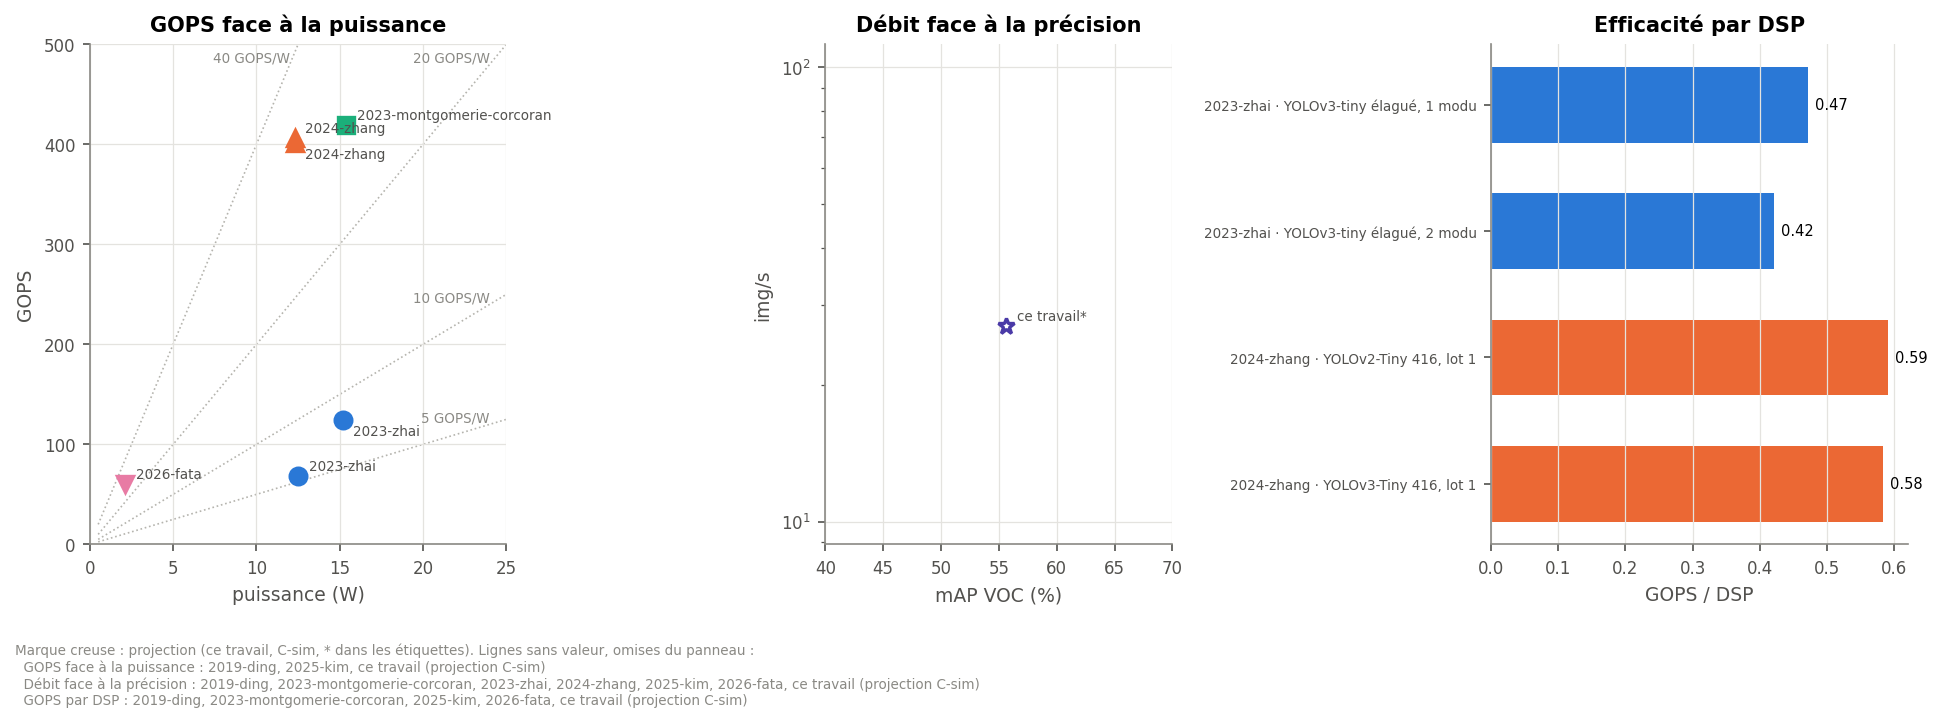
\includegraphics[width=\linewidth,height=0.42\textheight,keepaspectratio]{../../results/figures/resultats/etat_art.png}
\caption{Comparaison aux accélérateurs publiés : GOPS et puissance, débit et mAP, GOPS par DSP (marque creuse : projection de ce travail). (\texttt{etat\_art})}
\label{fig:etat_art}
% python -m tools.figures etat_art
\end{figure}}
\expandafter\def\csname artfig:graphe/graphe_tiny-yolov2-voc\endcsname{%
\begin{figure}[htbp]
\centering
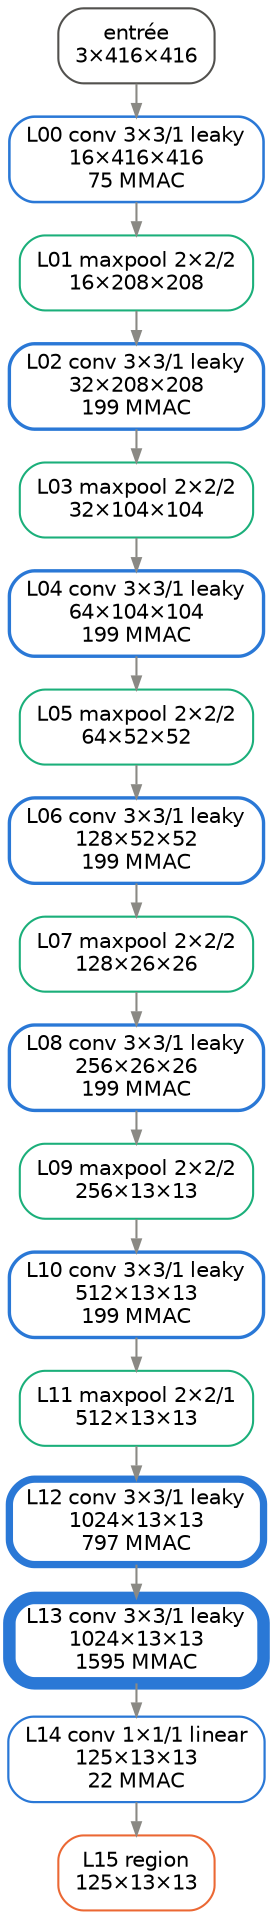
\includegraphics[width=\linewidth,height=0.42\textheight,keepaspectratio]{../../results/figures/modeles/graphe_tiny-yolov2-voc.png}
\caption{Graphe couche par couche (type, noyau et stride, forme de sortie C×H×W ; bord épais = beaucoup de MACs). (\texttt{graphe})}
\label{fig:graphe/graphe_tiny-yolov2-voc}
% python -m tools.figures graphe
\end{figure}}
\expandafter\def\csname artfig:fiche/fiche_tiny-yolov2-voc\endcsname{%
\begin{figure}[htbp]
\centering
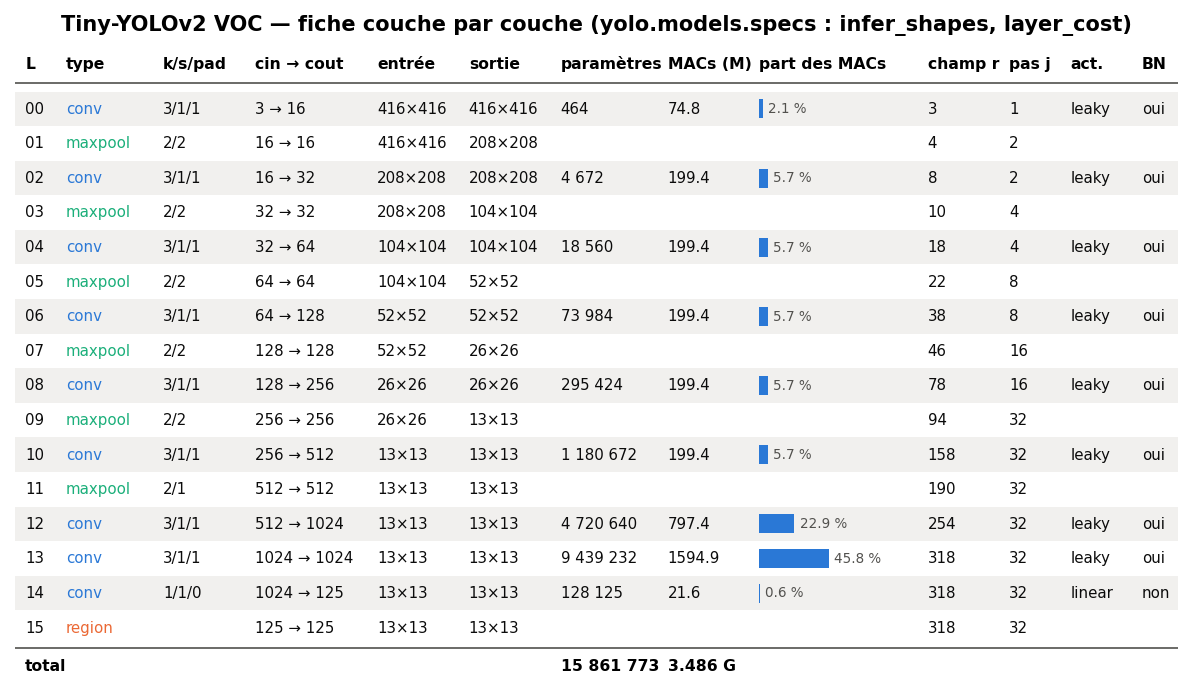
\includegraphics[width=\linewidth,height=0.42\textheight,keepaspectratio]{../../results/figures/reseaux/fiche_tiny-yolov2-voc.png}
\caption{Fiche couche par couche : type, noyau, formes, paramètres, MACs et leur part, champ réceptif et pas cumulé (CSV à côté de l'image). (\texttt{fiche})}
\label{fig:fiche/fiche_tiny-yolov2-voc}
% python -m tools.figures fiche
\end{figure}}
\expandafter\def\csname artfig:convolution\endcsname{%
\begin{figure}[htbp]
\centering
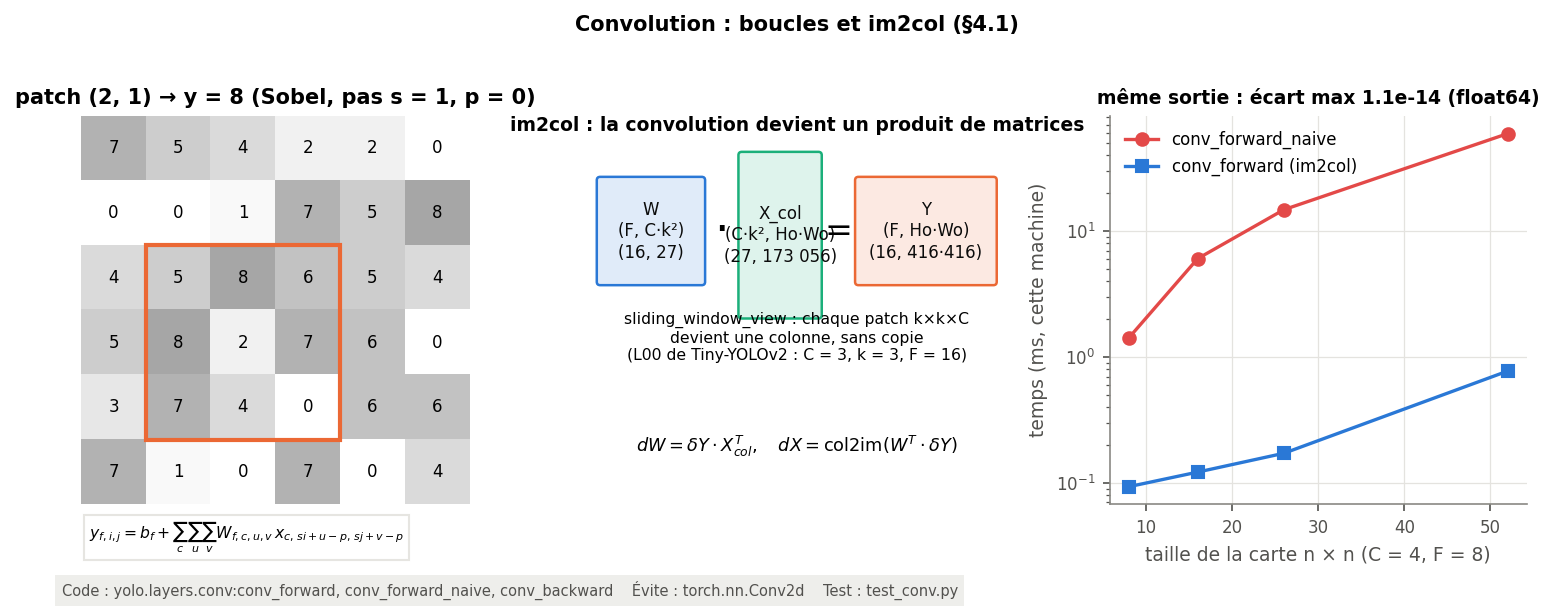
\includegraphics[width=\linewidth,height=0.42\textheight,keepaspectratio]{../../results/figures/maths/convolution.png}
\caption{Convolution : la formule sur un patch, le dépliage im2col en produit de matrices, et le temps des boucles face à im2col. (\texttt{convolution})}
\label{fig:convolution}
% python -m tools.figures convolution
\end{figure}}
\expandafter\def\csname artfig:retropropagation\endcsname{%
\begin{figure}[htbp]
\centering
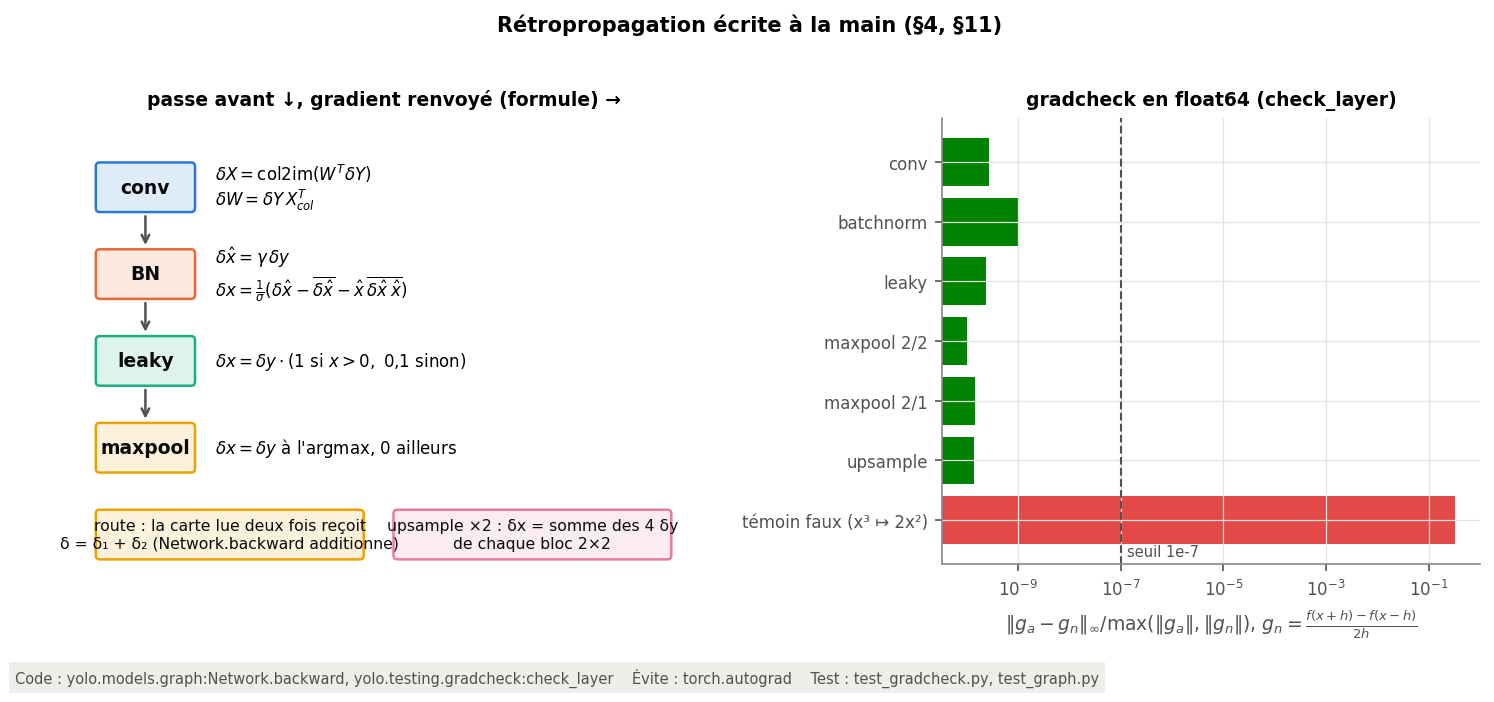
\includegraphics[width=\linewidth,height=0.42\textheight,keepaspectratio]{../../results/figures/maths/retropropagation.png}
\caption{Rétropropagation écrite à la main : formule du gradient renvoyé par chaque couche, puis l'erreur du gradcheck par couche face au seuil 1e-7. (\texttt{retropropagation})}
\label{fig:retropropagation}
% python -m tools.figures retropropagation
\end{figure}}
\expandafter\def\csname artfig:perte\endcsname{%
\begin{figure}[htbp]
\centering
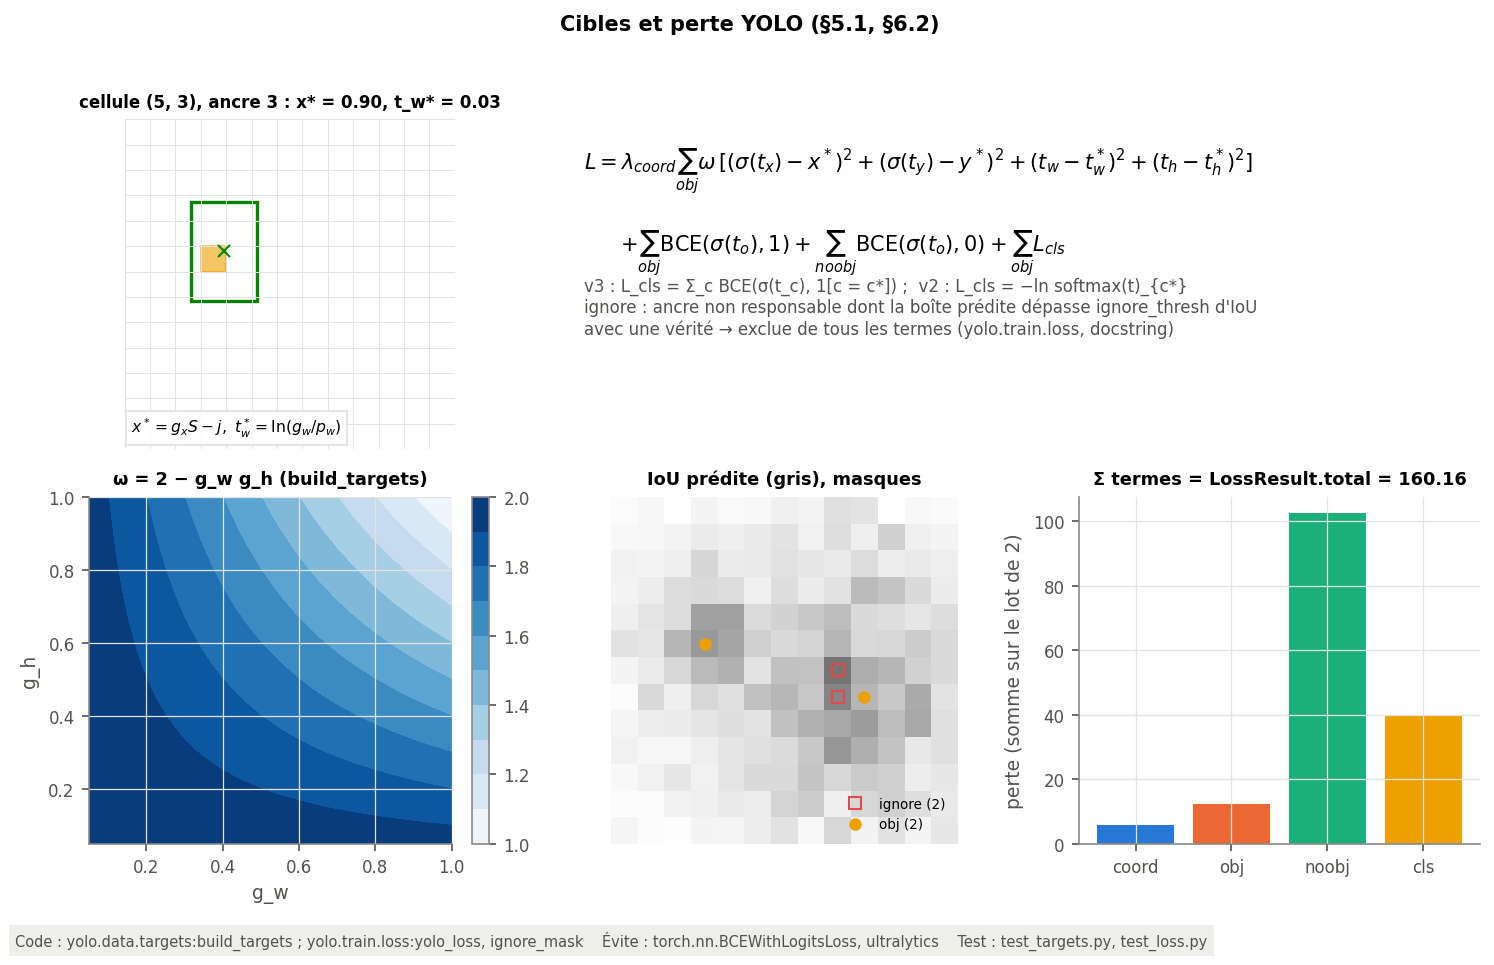
\includegraphics[width=\linewidth,height=0.42\textheight,keepaspectratio]{../../results/figures/maths/perte.png}
\caption{Cibles et perte YOLO : encodage d'une vérité, la perte terme par terme, le poids $\omega$ = 2 − g\_w g\_h, le masque ignore et la part de chaque terme sur un lot. (\texttt{perte})}
\label{fig:perte}
% python -m tools.figures perte
\end{figure}}
\expandafter\def\csname artfig:pr/pr_variantes\endcsname{%
\begin{figure}[htbp]
\centering
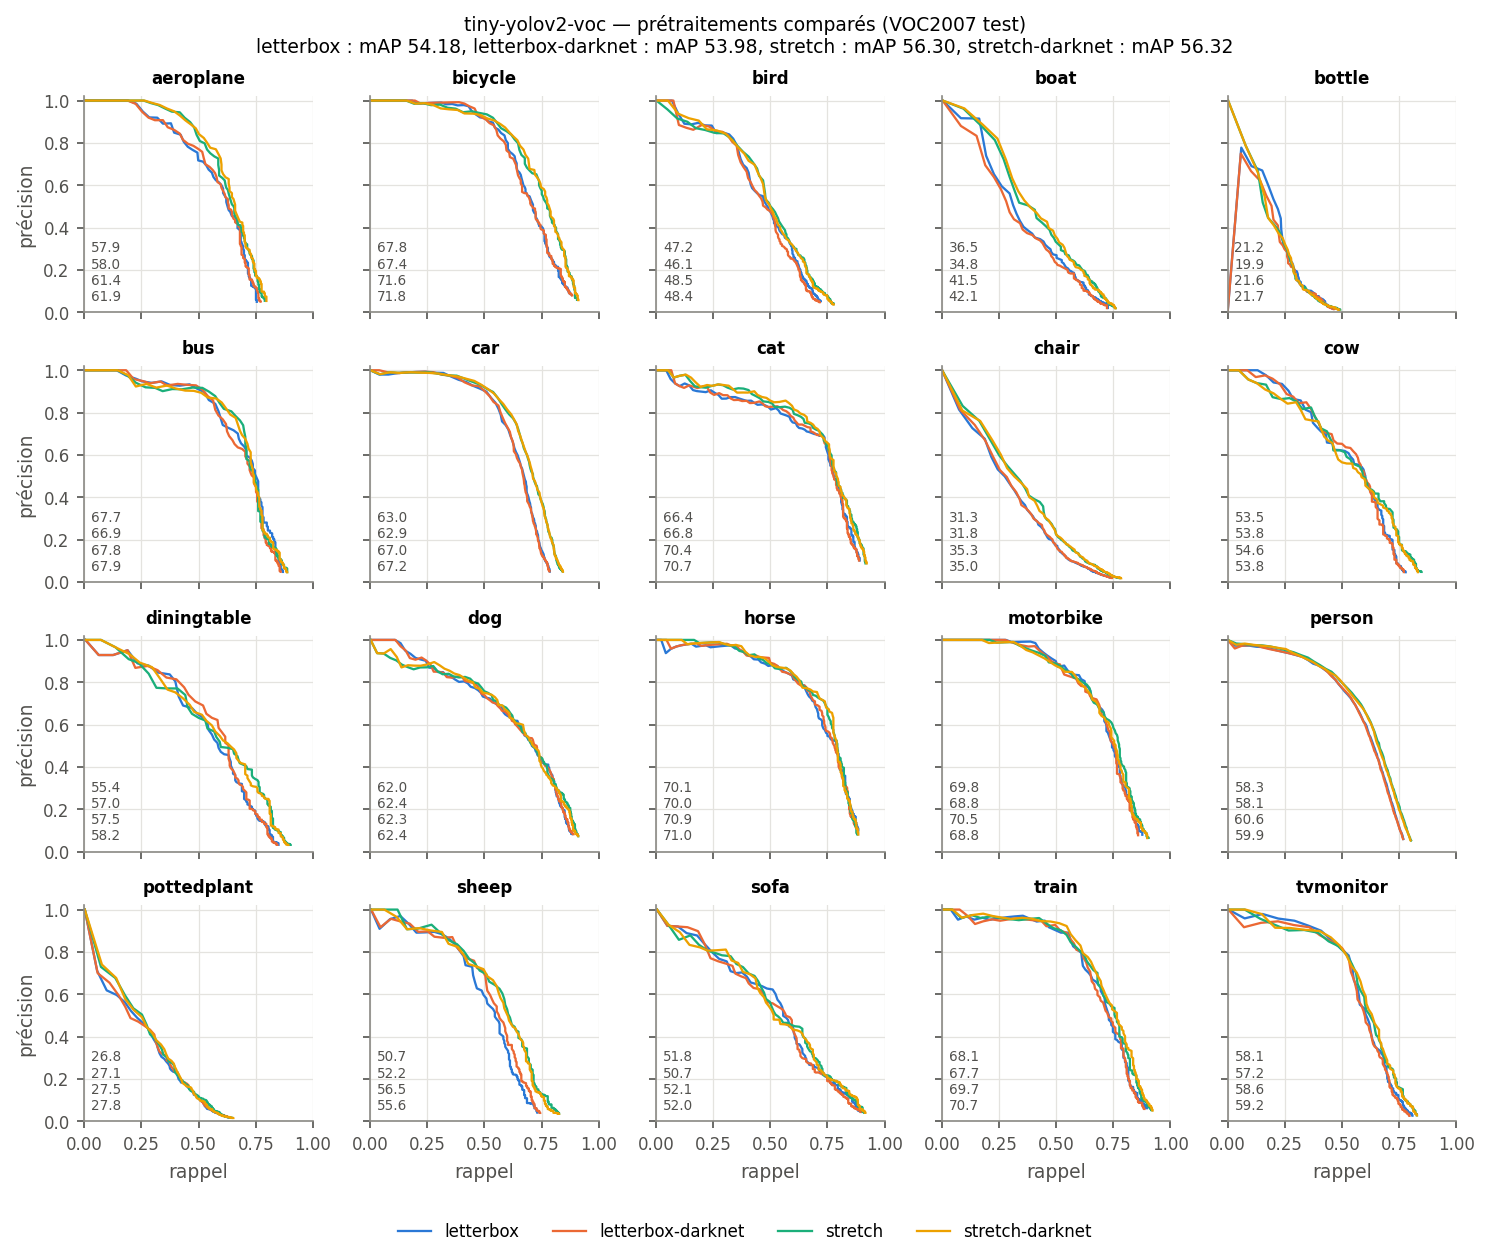
\includegraphics[width=\linewidth,height=0.42\textheight,keepaspectratio]{../../results/figures/resultats/pr_variantes.png}
\caption{Courbes précision-rappel par classe (11 points VOC07) pour chaque prétraitement évalué, puis les quatre superposées. (\texttt{pr})}
\label{fig:pr/pr_variantes}
% python -m tools.figures pr
\end{figure}}
\expandafter\def\csname artfig:nms_map\endcsname{%
\begin{figure}[htbp]
\centering
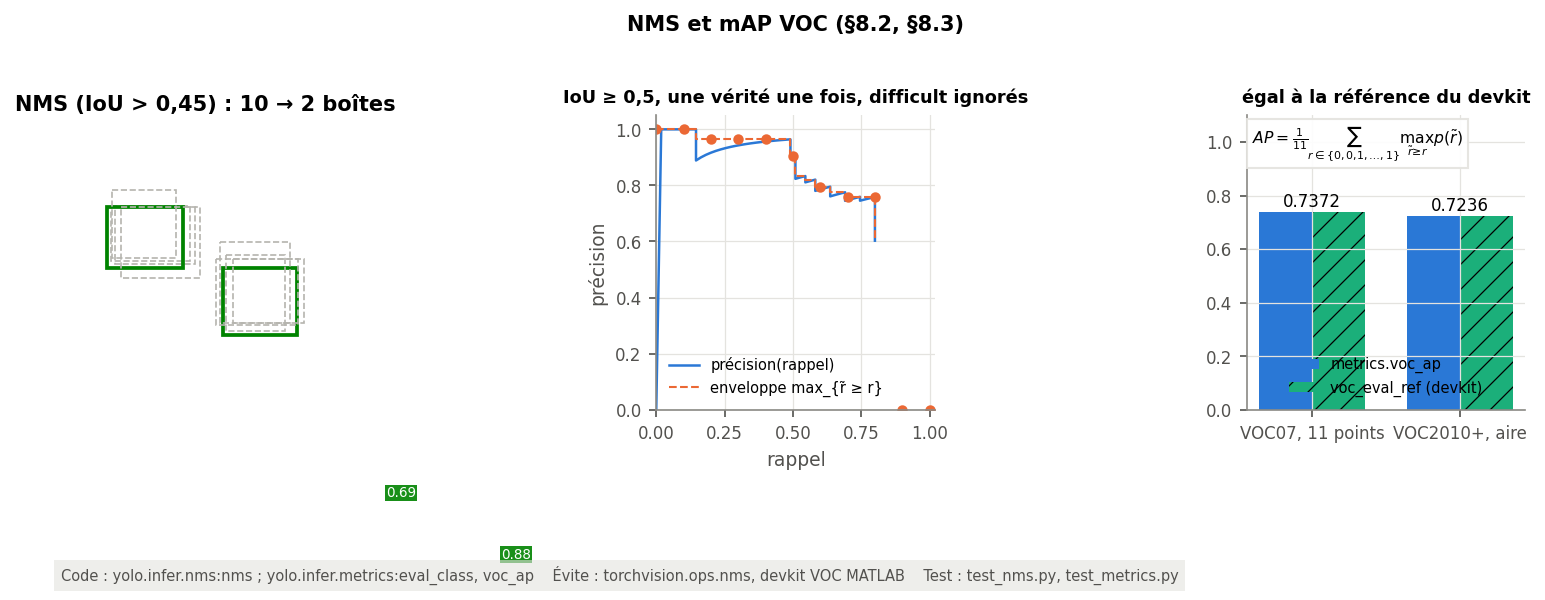
\includegraphics[width=\linewidth,height=0.42\textheight,keepaspectratio]{../../results/figures/maths/nms_map.png}
\caption{NMS pas à pas, appariement détections / vérités et courbe précision-rappel, AP VOC07 sur 11 points face à l'aire sous l'enveloppe, égale à la référence du devkit. (\texttt{nms\_map})}
\label{fig:nms_map}
% python -m tools.figures nms_map
\end{figure}}
\expandafter\def\csname artfig:quantification\endcsname{%
\begin{figure}[htbp]
\centering
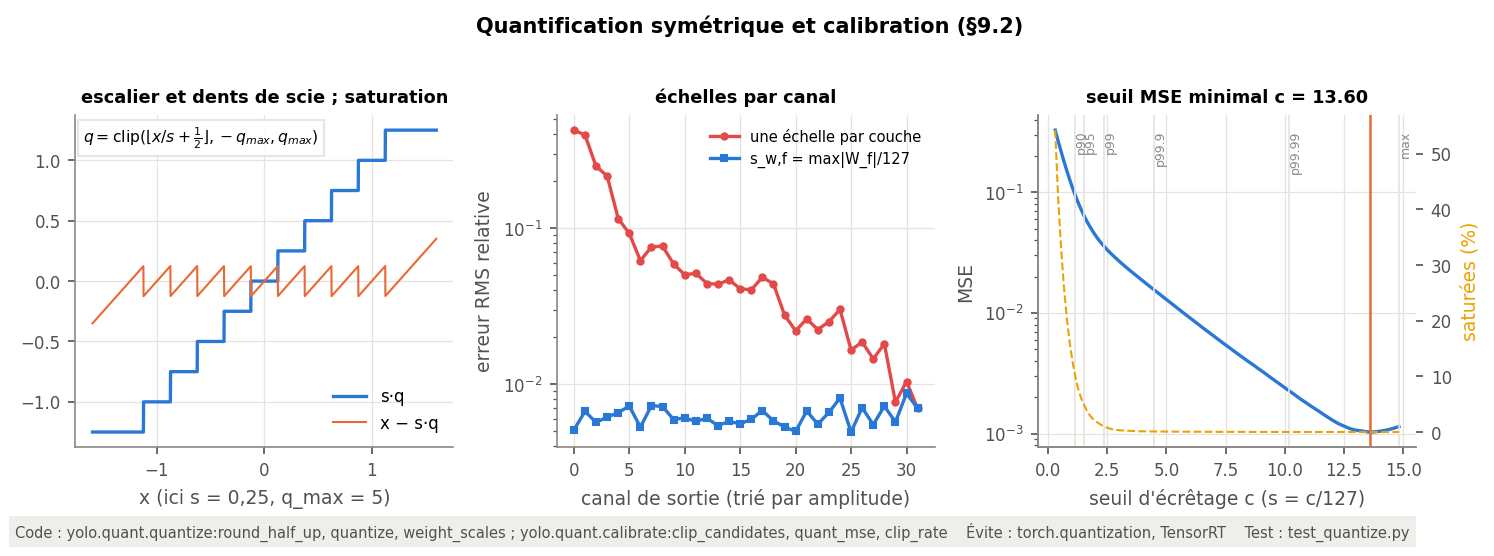
\includegraphics[width=\linewidth,height=0.42\textheight,keepaspectratio]{../../results/figures/maths/quantification.png}
\caption{Quantification symétrique : l'escalier et son erreur, échelles par canal face à une échelle par couche, choix du seuil d'écrêtage par la MSE. (\texttt{quantification})}
\label{fig:quantification}
% python -m tools.figures quantification
\end{figure}}
\expandafter\def\csname artfig:entier\endcsname{%
\begin{figure}[htbp]
\centering
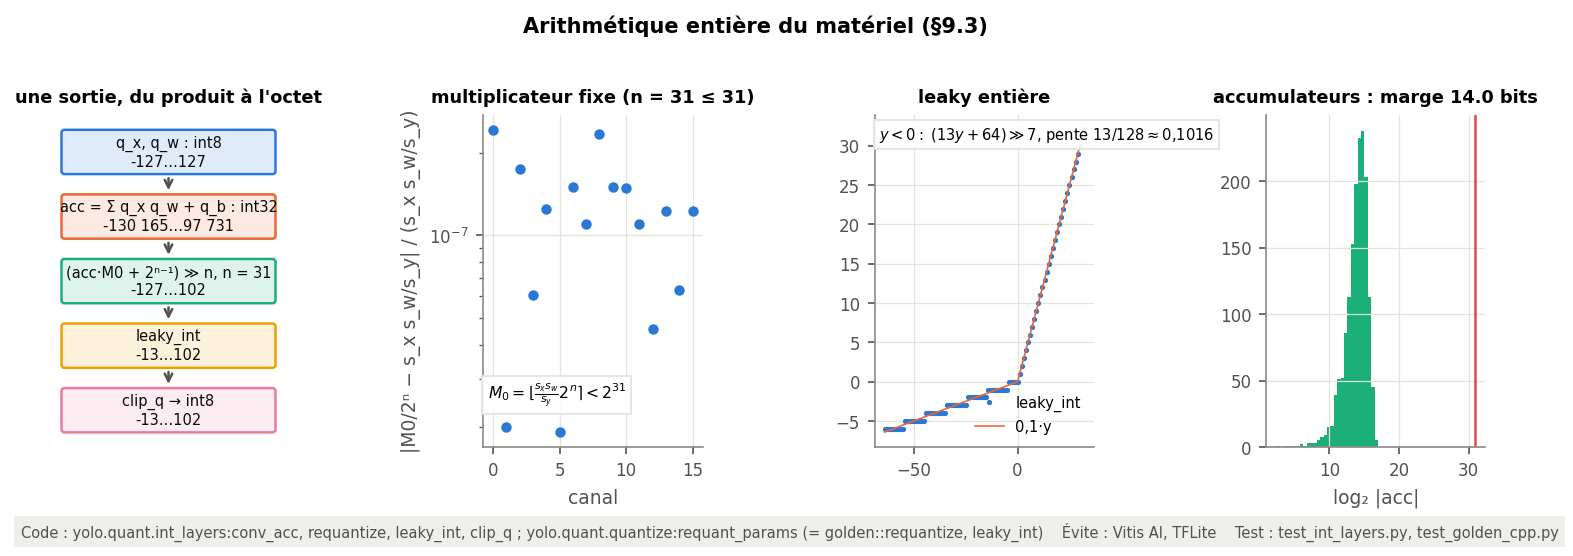
\includegraphics[width=\linewidth,height=0.42\textheight,keepaspectratio]{../../results/figures/maths/entier.png}
\caption{Arithmétique entière du matériel : chaîne d'une sortie, multiplicateur fixe M0/2$^n$, leaky entière 13/128 et marge des accumulateurs int32. (\texttt{entier})}
\label{fig:entier}
% python -m tools.figures entier
\end{figure}}
\expandafter\def\csname artfig:calibration/calibration_tiny-yolov2-voc\endcsname{%
\begin{figure}[htbp]
\centering
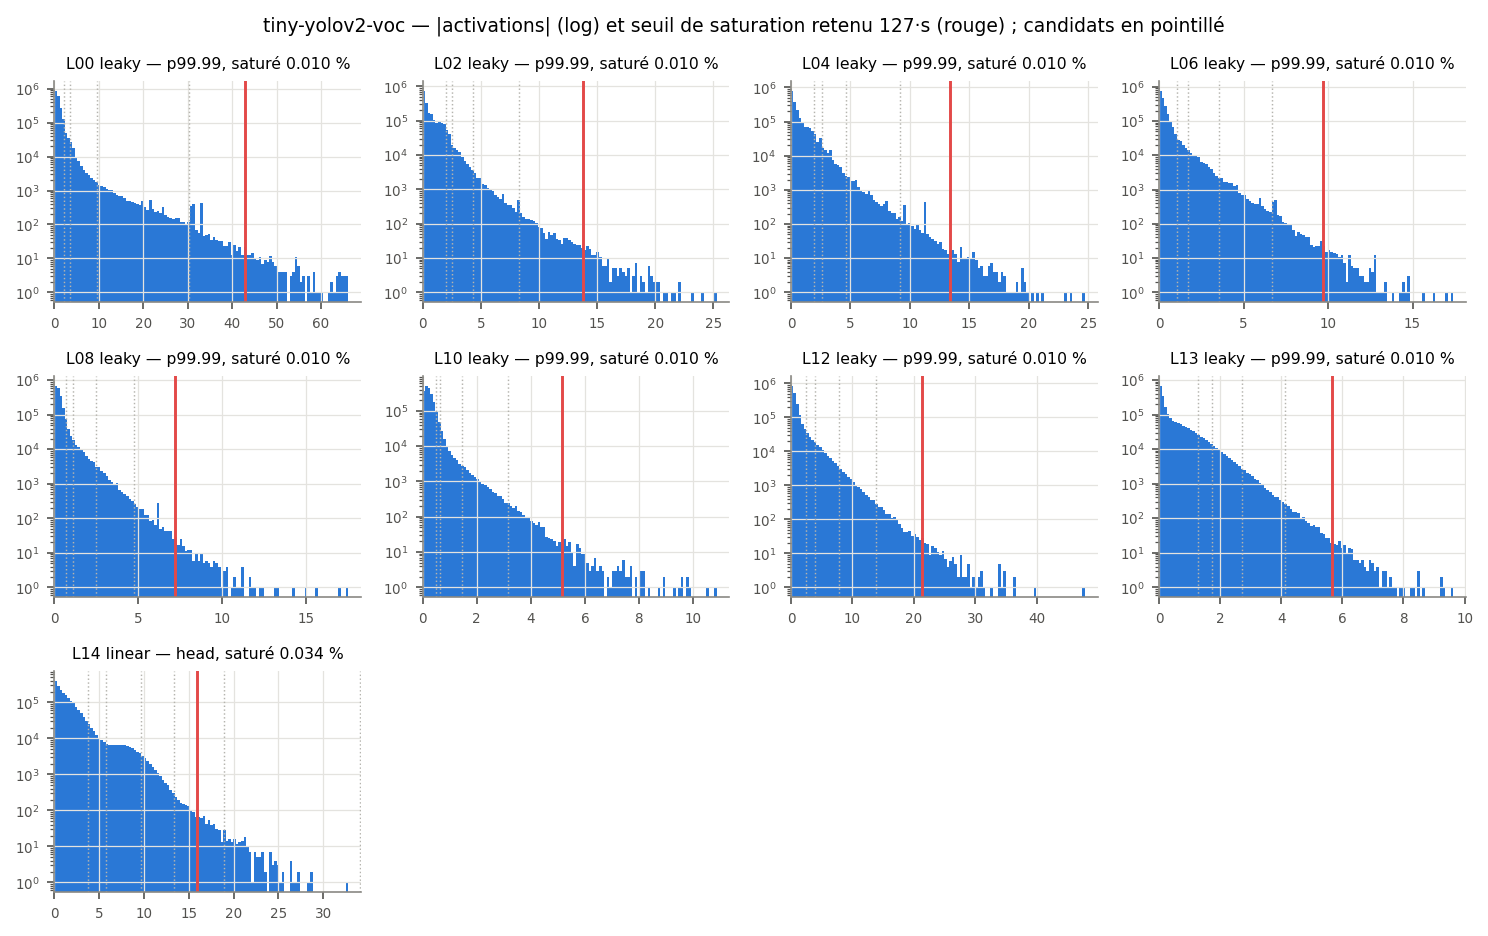
\includegraphics[width=\linewidth,height=0.42\textheight,keepaspectratio]{../../results/figures/resultats/calibration_tiny-yolov2-voc.png}
\caption{Distribution des activations par couche et seuil de saturation retenu par la calibration ; échelles des poids par canal. (\texttt{calibration})}
\label{fig:calibration/calibration_tiny-yolov2-voc}
% python -m tools.figures calibration
\end{figure}}
\expandafter\def\csname artfig:erreur_couches/erreur_couches_tiny-yolov2-voc\endcsname{%
\begin{figure}[htbp]
\centering
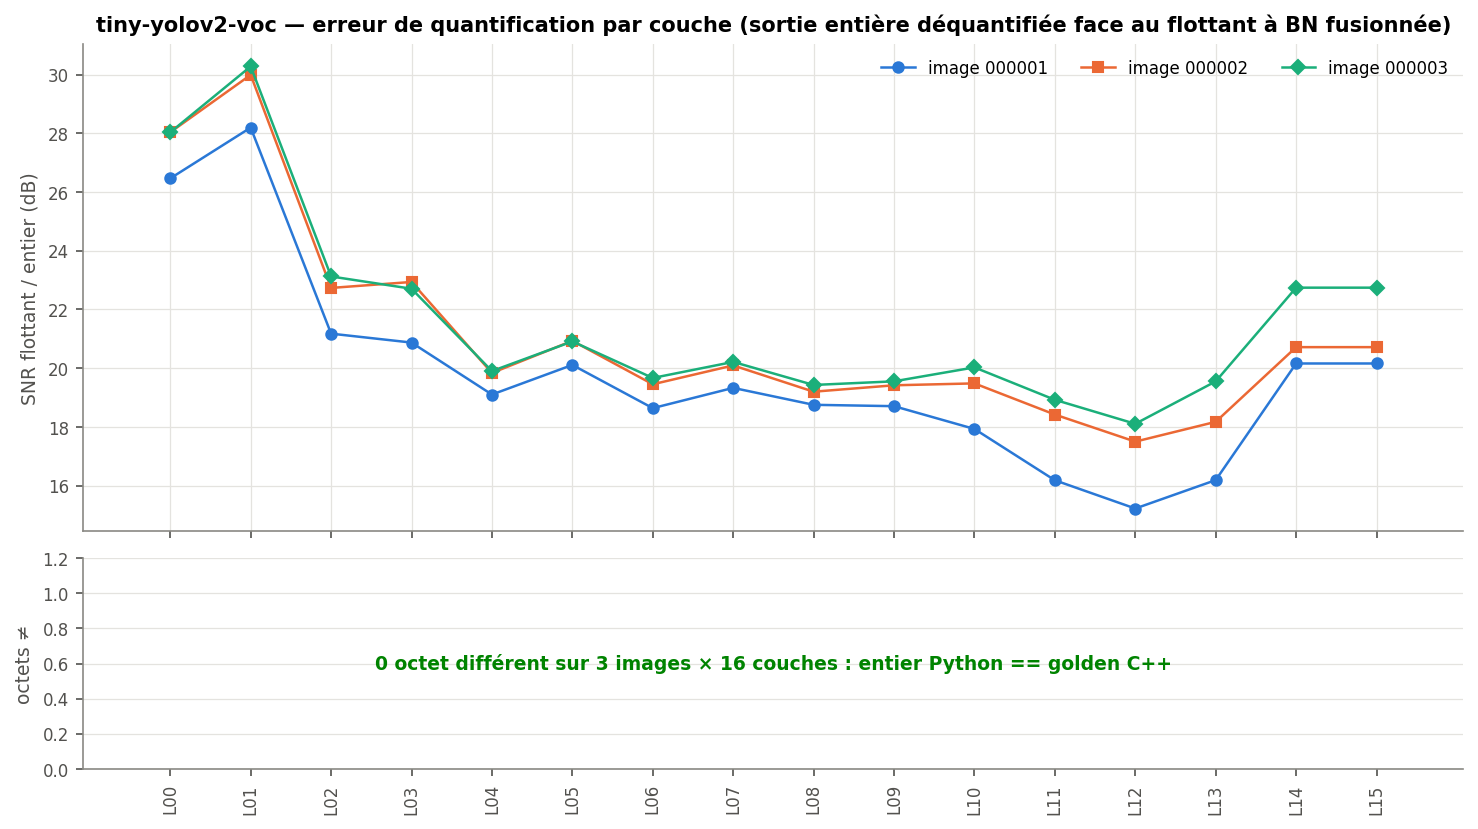
\includegraphics[width=\linewidth,height=0.42\textheight,keepaspectratio]{../../results/figures/resultats/erreur_couches_tiny-yolov2-voc.png}
\caption{SNR par couche entre le flottant et l'entier déquantifié, et écart entier Python $\leftrightarrow$ golden C++ (0 partout : bit-exact). (\texttt{erreur\_couches})}
\label{fig:erreur_couches/erreur_couches_tiny-yolov2-voc}
% python -m tools.figures erreur_couches
\end{figure}}
\expandafter\def\csname artfig:chaine_verif\endcsname{%
\begin{figure}[htbp]
\centering
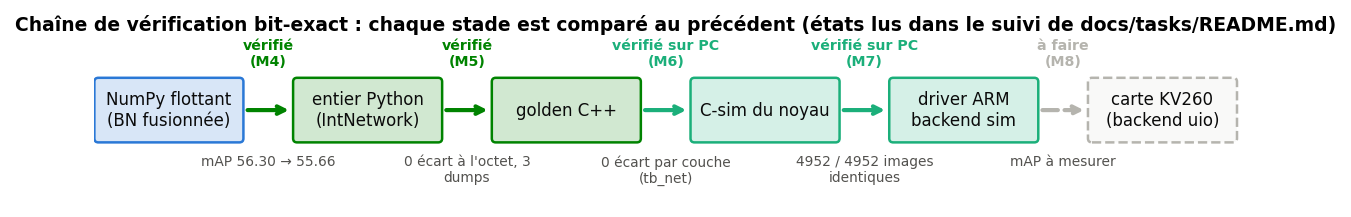
\includegraphics[width=\linewidth,height=0.42\textheight,keepaspectratio]{../../results/figures/materiel/chaine_verif.png}
\caption{Chaîne de vérification bit-exact, du flottant NumPy à la carte : critère et état de chaque passage. (\texttt{chaine\_verif})}
\label{fig:chaine_verif}
% python -m tools.figures chaine_verif
\end{figure}}
\expandafter\def\csname artfig:moteur\endcsname{%
\begin{figure}[htbp]
\centering
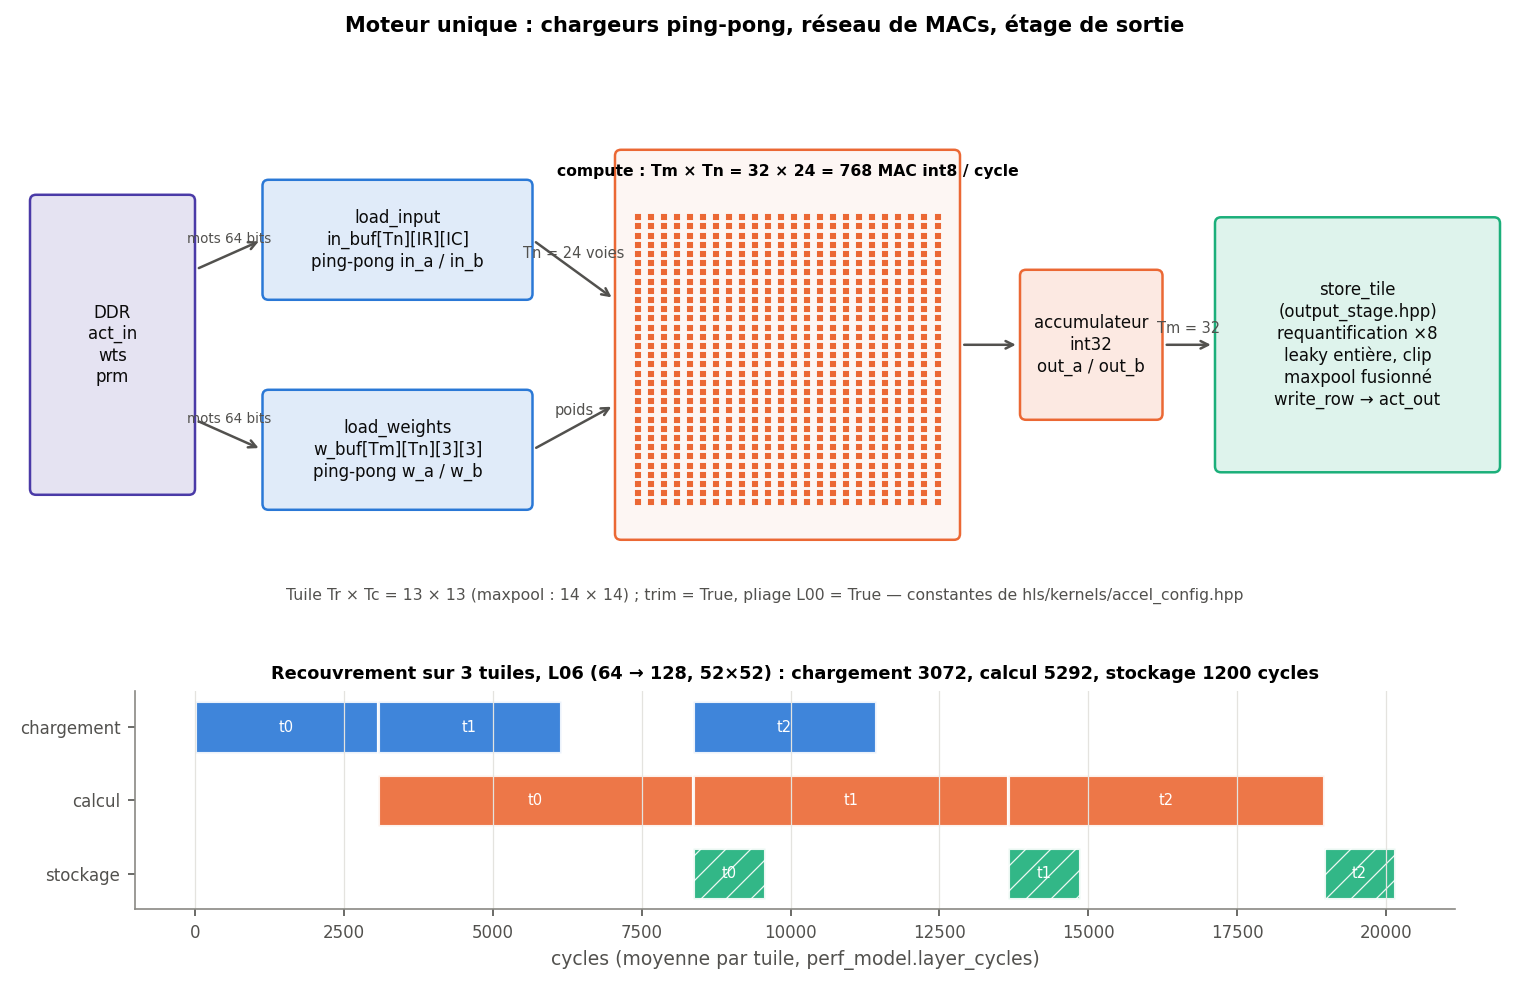
\includegraphics[width=\linewidth,height=0.42\textheight,keepaspectratio]{../../results/figures/materiel/moteur.png}
\caption{Moteur unique : chargeurs ping-pong, réseau Tm × Tn de MACs, accumulateur, étage de sortie, et chronogramme du recouvrement sur 3 tuiles. (\texttt{moteur})}
\label{fig:moteur}
% python -m tools.figures moteur
\end{figure}}
\expandafter\def\csname artfig:tuilage\endcsname{%
\begin{figure}[htbp]
\centering
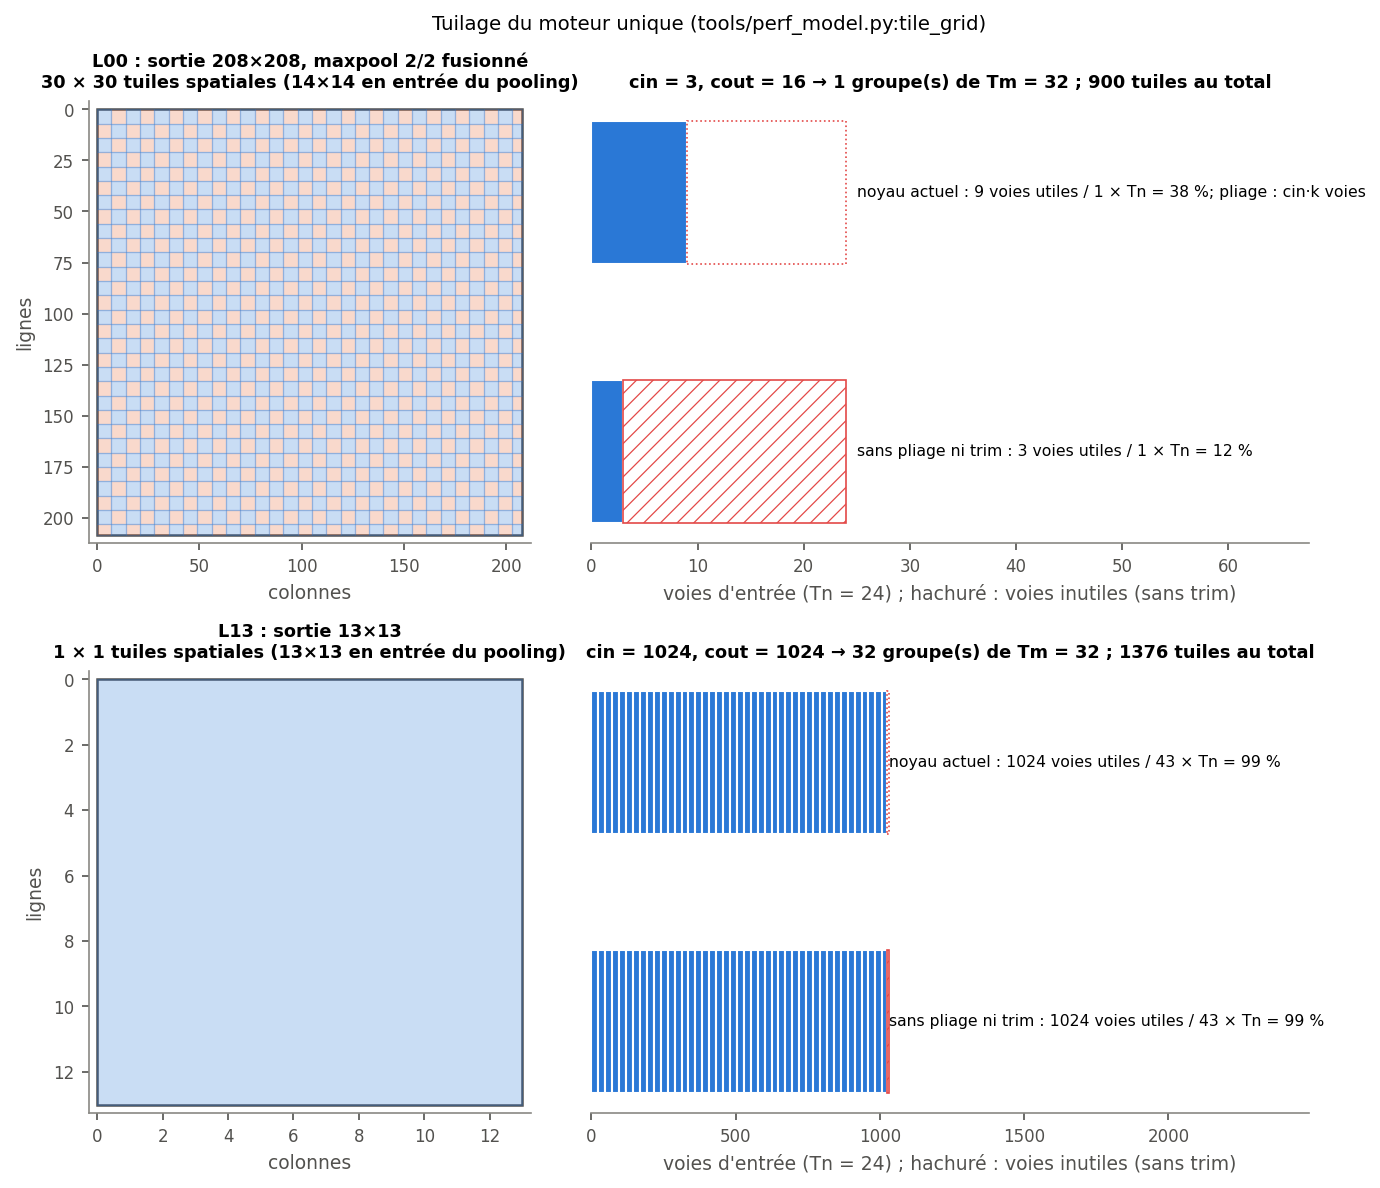
\includegraphics[width=\linewidth,height=0.42\textheight,keepaspectratio]{../../results/figures/materiel/tuilage.png}
\caption{Tuilage de deux couches : tuiles spatiales et voies d'entrée, avec le pliage de L00 (cin = 3) et la couche 13×13 couverte par une seule tuile. (\texttt{tuilage})}
\label{fig:tuilage}
% python -m tools.figures tuilage
\end{figure}}
\expandafter\def\csname artfig:soc\endcsname{%
\begin{figure}[htbp]
\centering
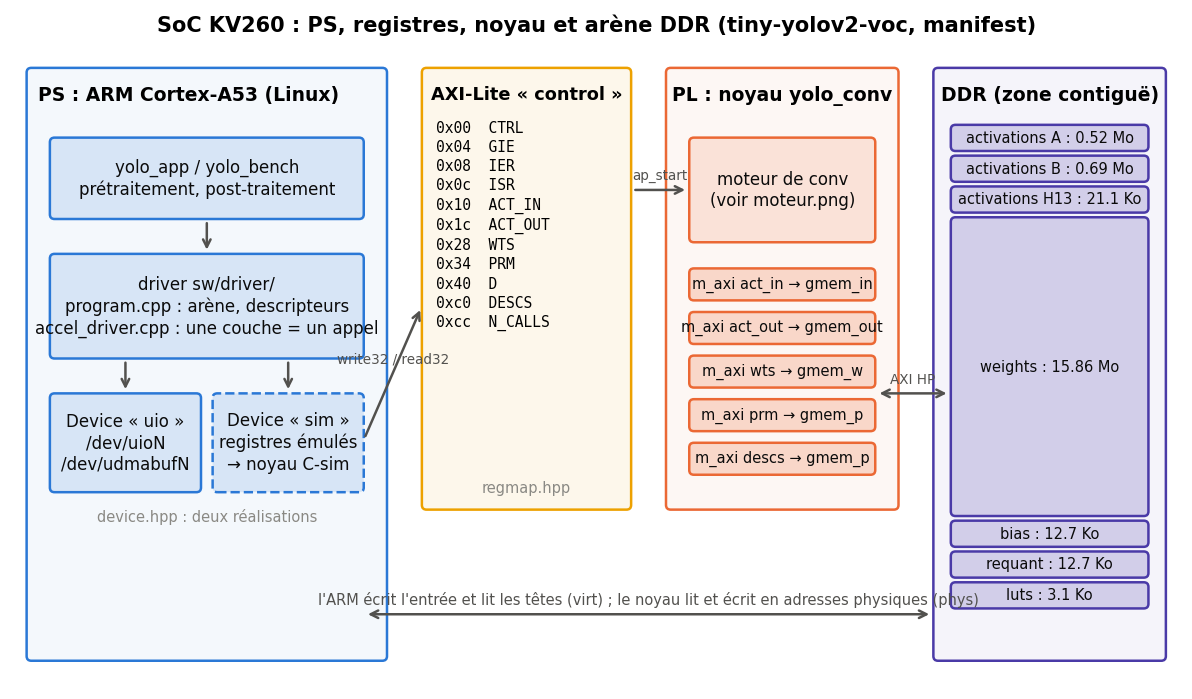
\includegraphics[width=\linewidth,height=0.42\textheight,keepaspectratio]{../../results/figures/materiel/soc.png}
\caption{Schéma du SoC : application et driver sur l'ARM, registres AXI-Lite, ports m\_axi du noyau et découpage de l'arène DDR. (\texttt{soc})}
\label{fig:soc}
% python -m tools.figures soc
\end{figure}}
\expandafter\def\csname artfig:cascade_m10\endcsname{%
\begin{figure}[htbp]
\centering
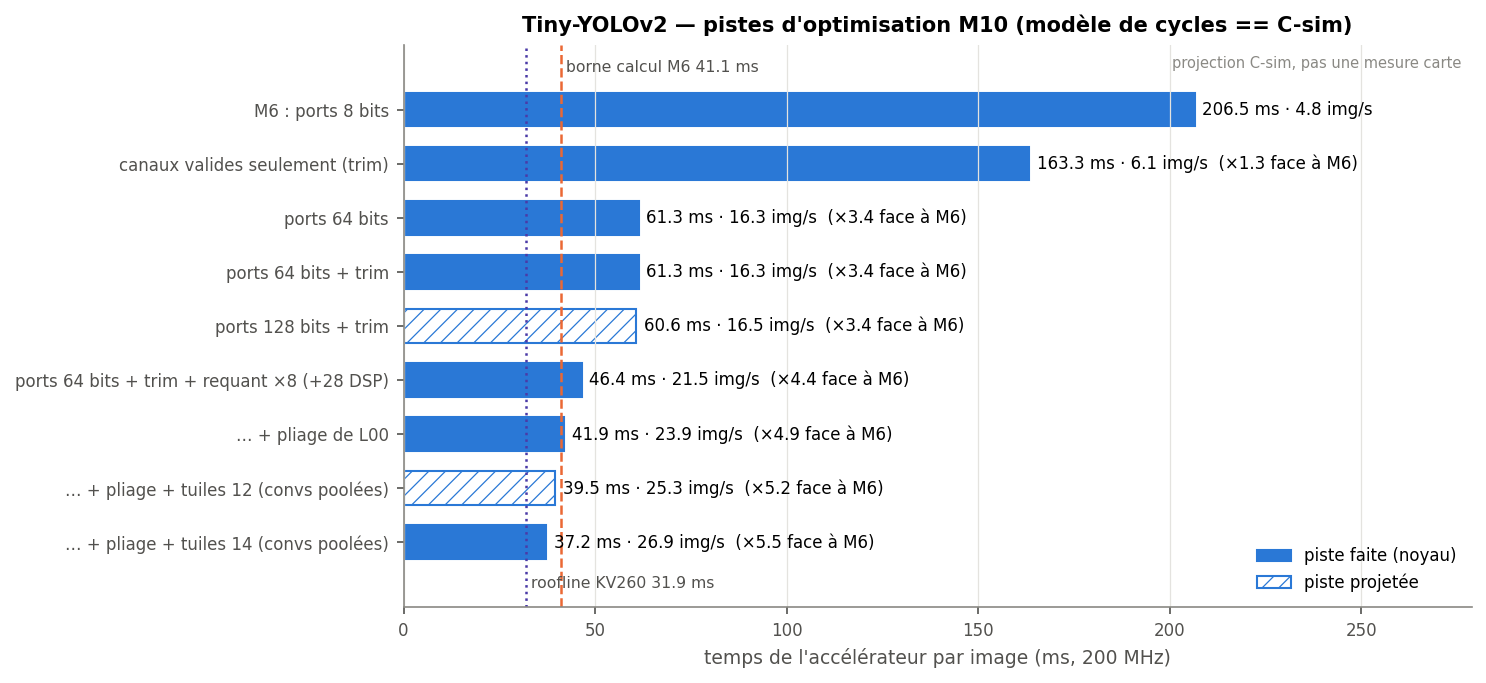
\includegraphics[width=\linewidth,height=0.42\textheight,keepaspectratio]{../../results/figures/resultats/cascade_m10.png}
\caption{Temps par image de Tiny-YOLOv2 à chaque piste d'optimisation M10, face à la borne de calcul et au roofline KV260. (\texttt{cascade\_m10})}
\label{fig:cascade_m10}
% python -m tools.figures cascade_m10
\end{figure}}
\expandafter\def\csname artfig:roofline_couches/roofline_couches_kv260\endcsname{%
\begin{figure}[htbp]
\centering
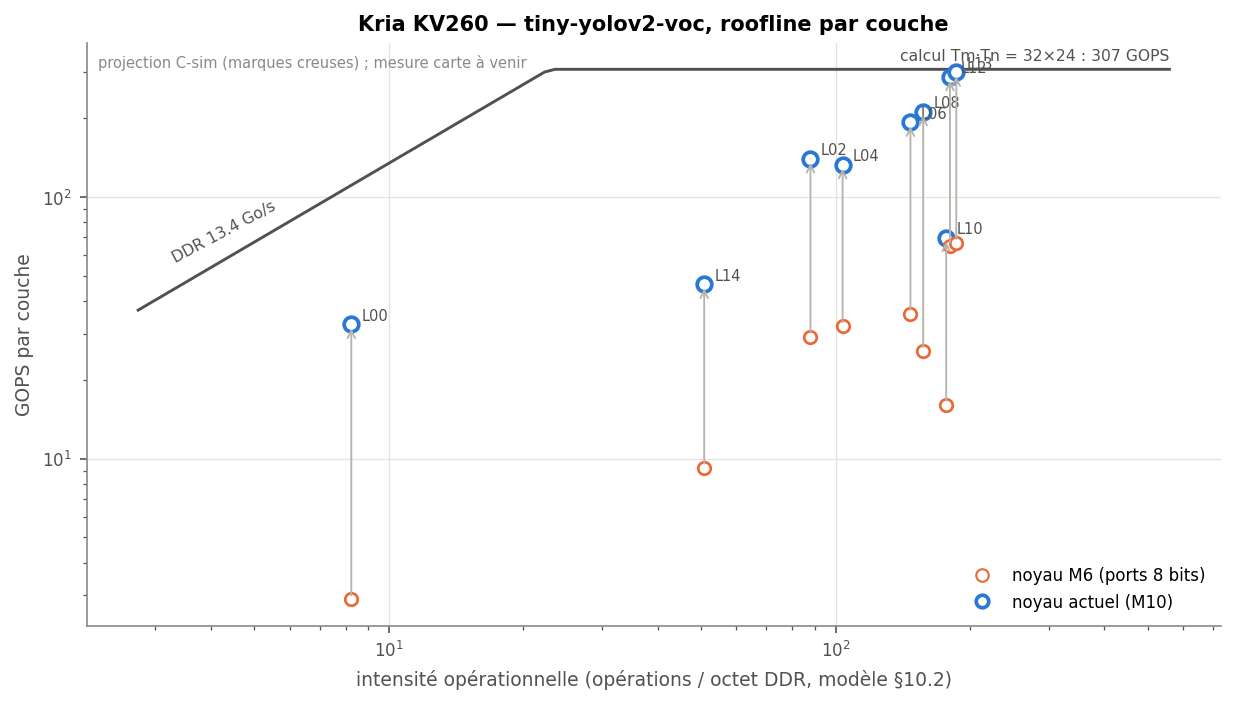
\includegraphics[width=\linewidth,height=0.42\textheight,keepaspectratio]{../../results/figures/resultats/roofline_couches_kv260.png}
\caption{Roofline KV260 avec un point par couche de Tiny-YOLOv2, avant et après les optimisations M10. (\texttt{roofline\_couches})}
\label{fig:roofline_couches/roofline_couches_kv260}
% python -m tools.figures roofline_couches
\end{figure}}
\expandafter\def\csname artfig:cycles_couches\endcsname{%
\begin{figure}[htbp]
\centering
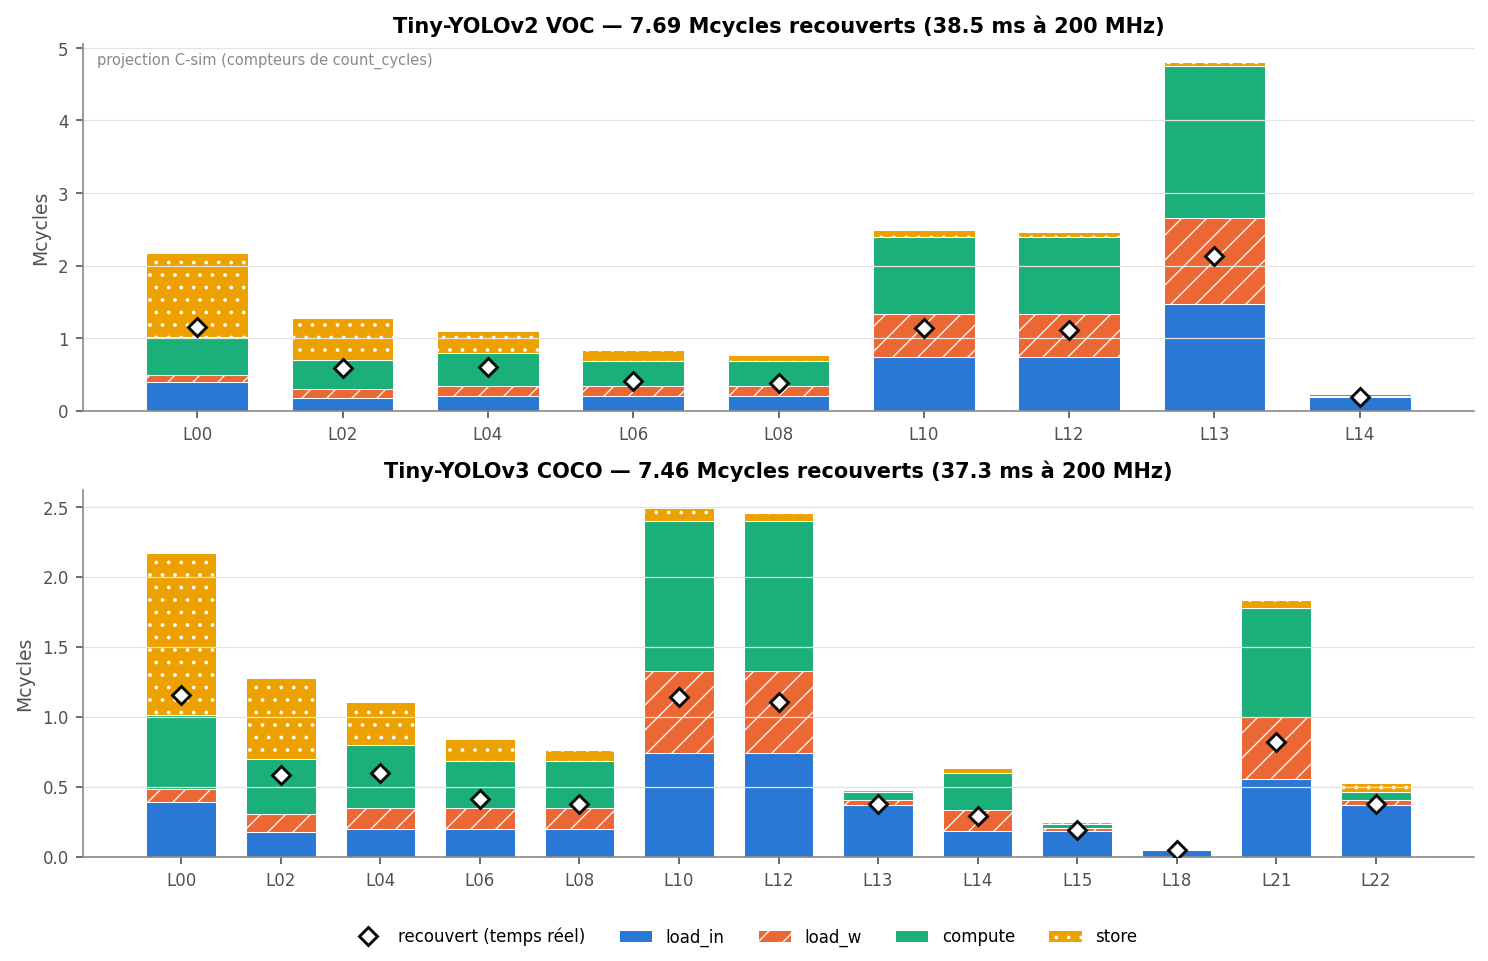
\includegraphics[width=\linewidth,height=0.42\textheight,keepaspectratio]{../../results/figures/resultats/cycles_couches.png}
\caption{Cycles par couche du noyau actuel, décomposés en chargements, calcul et stockage ; le losange donne le temps réel avec recouvrement. (\texttt{cycles\_couches})}
\label{fig:cycles_couches}
% python -m tools.figures cycles_couches
\end{figure}}
\expandafter\def\csname artfig:map_stades\endcsname{%
\begin{figure}[htbp]
\centering
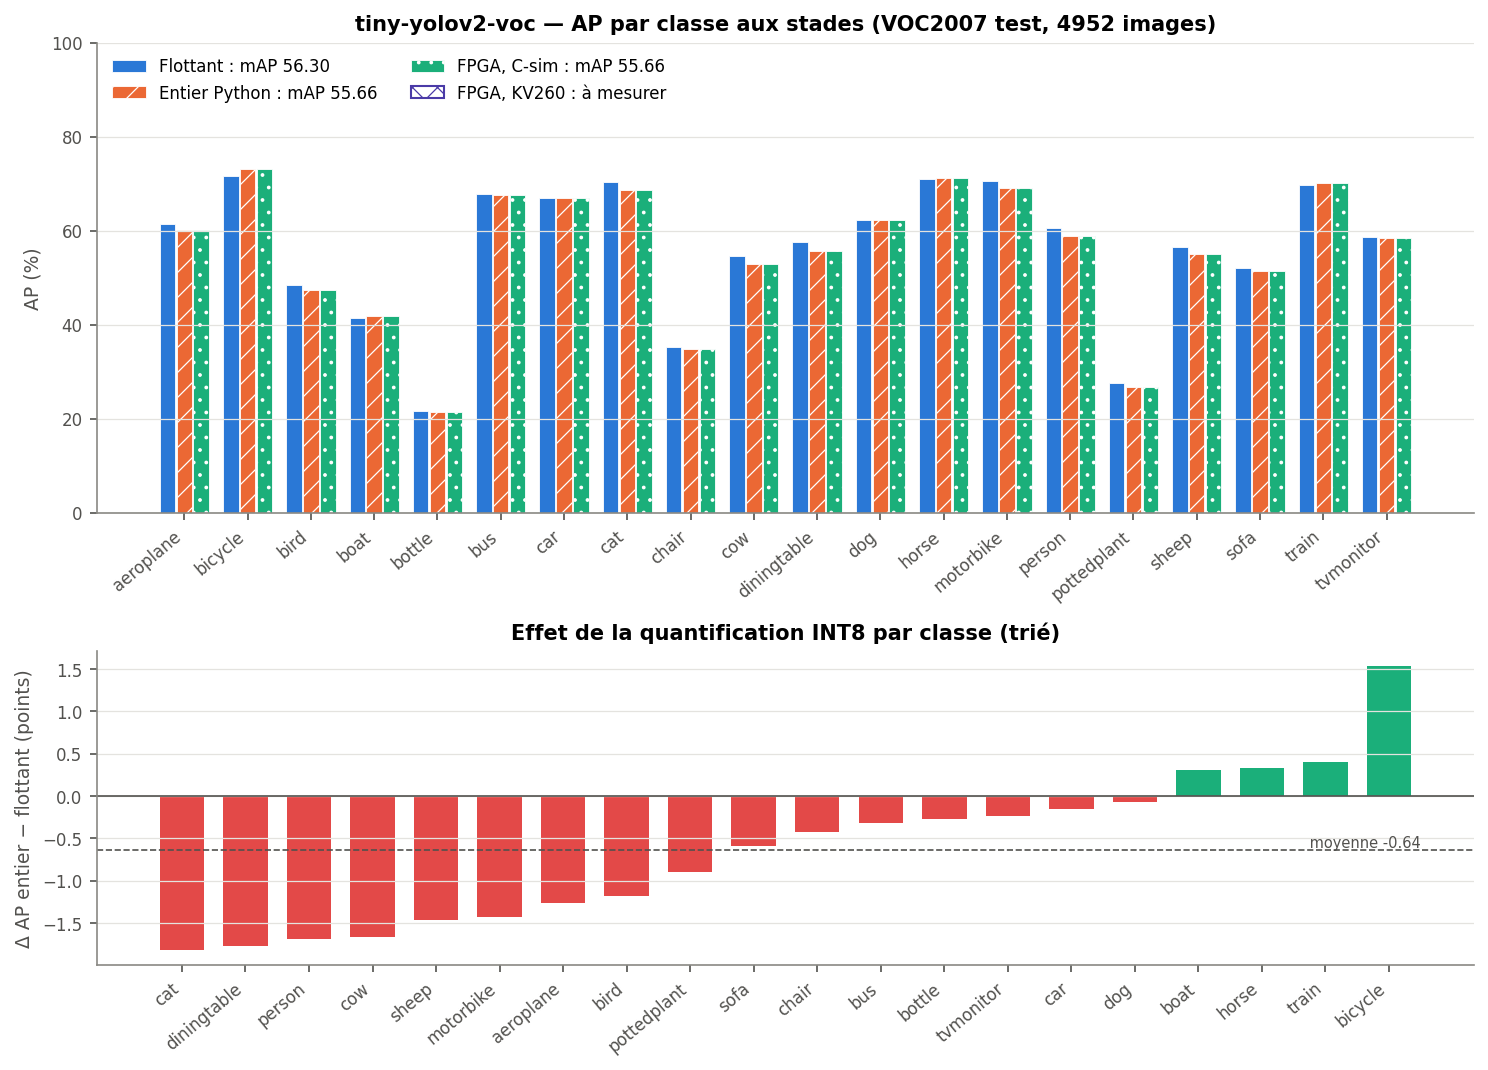
\includegraphics[width=\linewidth,height=0.42\textheight,keepaspectratio]{../../results/figures/resultats/map_stades.png}
\caption{AP par classe aux stades flottant, entier et C-sim (la carte quand elle sera mesurée), et écart entier − flottant trié. (\texttt{map\_stades})}
\label{fig:map_stades}
% python -m tools.figures map_stades
\end{figure}}
\expandafter\def\csname artfig:ressources\endcsname{%
\begin{figure}[htbp]
\centering
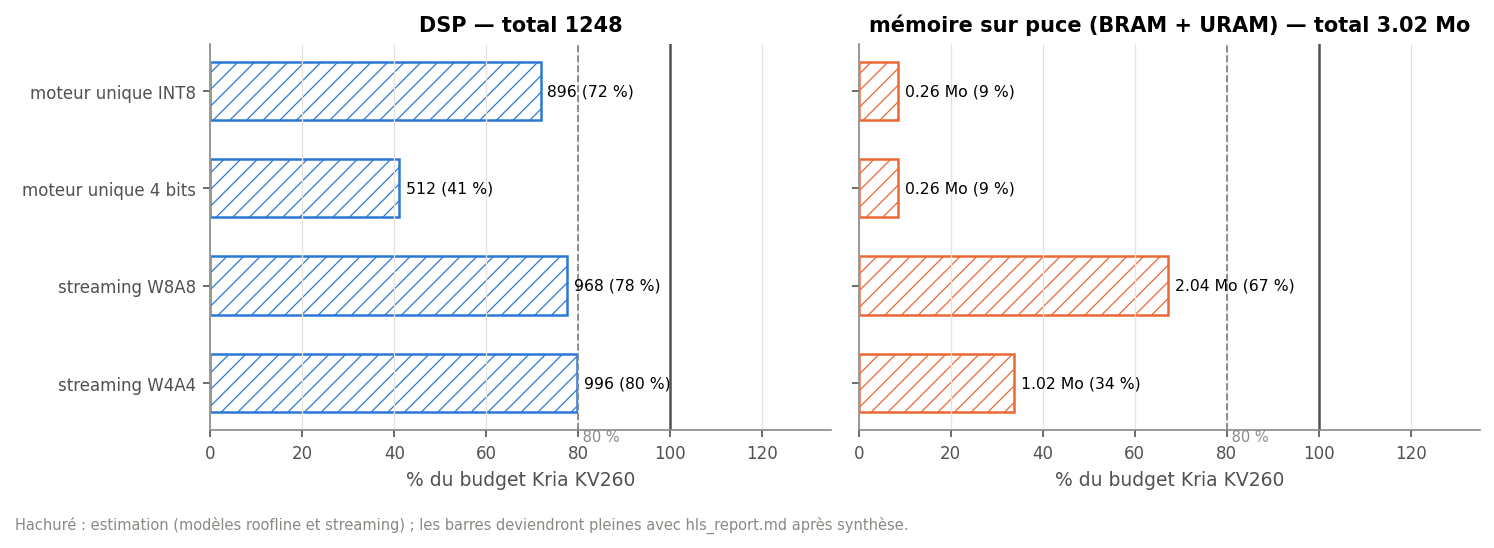
\includegraphics[width=\linewidth,height=0.42\textheight,keepaspectratio]{../../results/figures/resultats/ressources.png}
\caption{DSP, mémoire sur puce et LUT des architectures (moteur unique INT8, pow2 et 4 bits, streaming) face au budget de la KV260 ; hachuré : estimation, plein : synthèse. (\texttt{ressources})}
\label{fig:ressources}
% python -m tools.figures ressources
\end{figure}}
\expandafter\def\csname artfig:hw_postproc\endcsname{%
\begin{figure}[htbp]
\centering
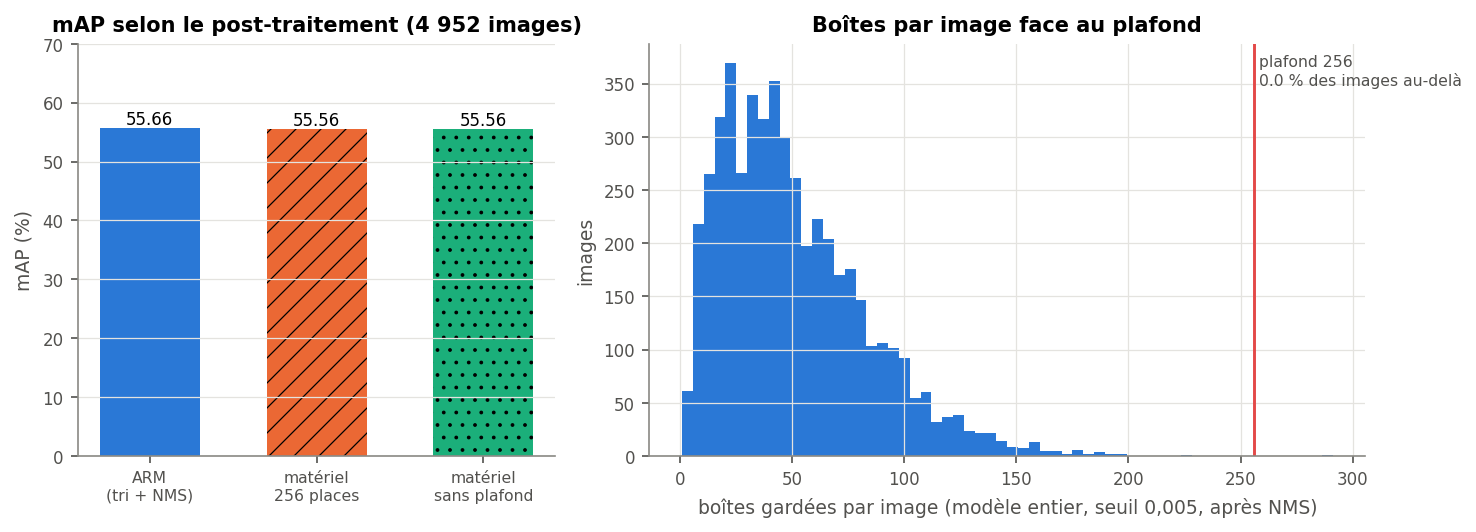
\includegraphics[width=\linewidth,height=0.42\textheight,keepaspectratio]{../../results/figures/resultats/hw_postproc.png}
\caption{mAP avec le post-traitement matériel, avec et sans plafond de boîtes, et nombre de boîtes par image face au plafond. (\texttt{hw\_postproc})}
\label{fig:hw_postproc}
% python -m tools.figures hw_postproc
\end{figure}}
\expandafter\def\csname artfig:map_formats\endcsname{%
\begin{figure}[htbp]
\centering
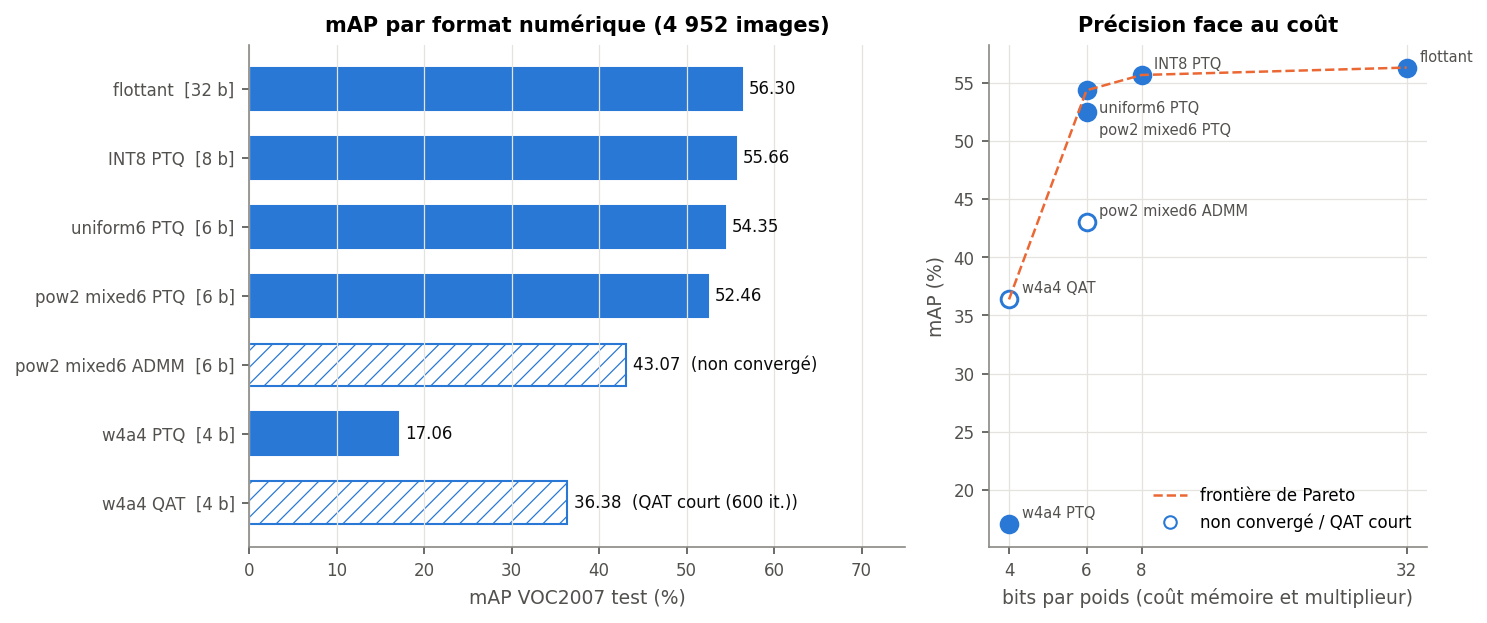
\includegraphics[width=\linewidth,height=0.42\textheight,keepaspectratio]{../../results/figures/resultats/map_formats.png}
\caption{mAP de Tiny-YOLOv2 selon le format des poids (flottant, INT8, puissances de 2, 4 bits), et frontière précision / bits. (\texttt{map\_formats})}
\label{fig:map_formats}
% python -m tools.figures map_formats
\end{figure}}
\expandafter\def\csname artfig:streaming\endcsname{%
\begin{figure}[htbp]
\centering
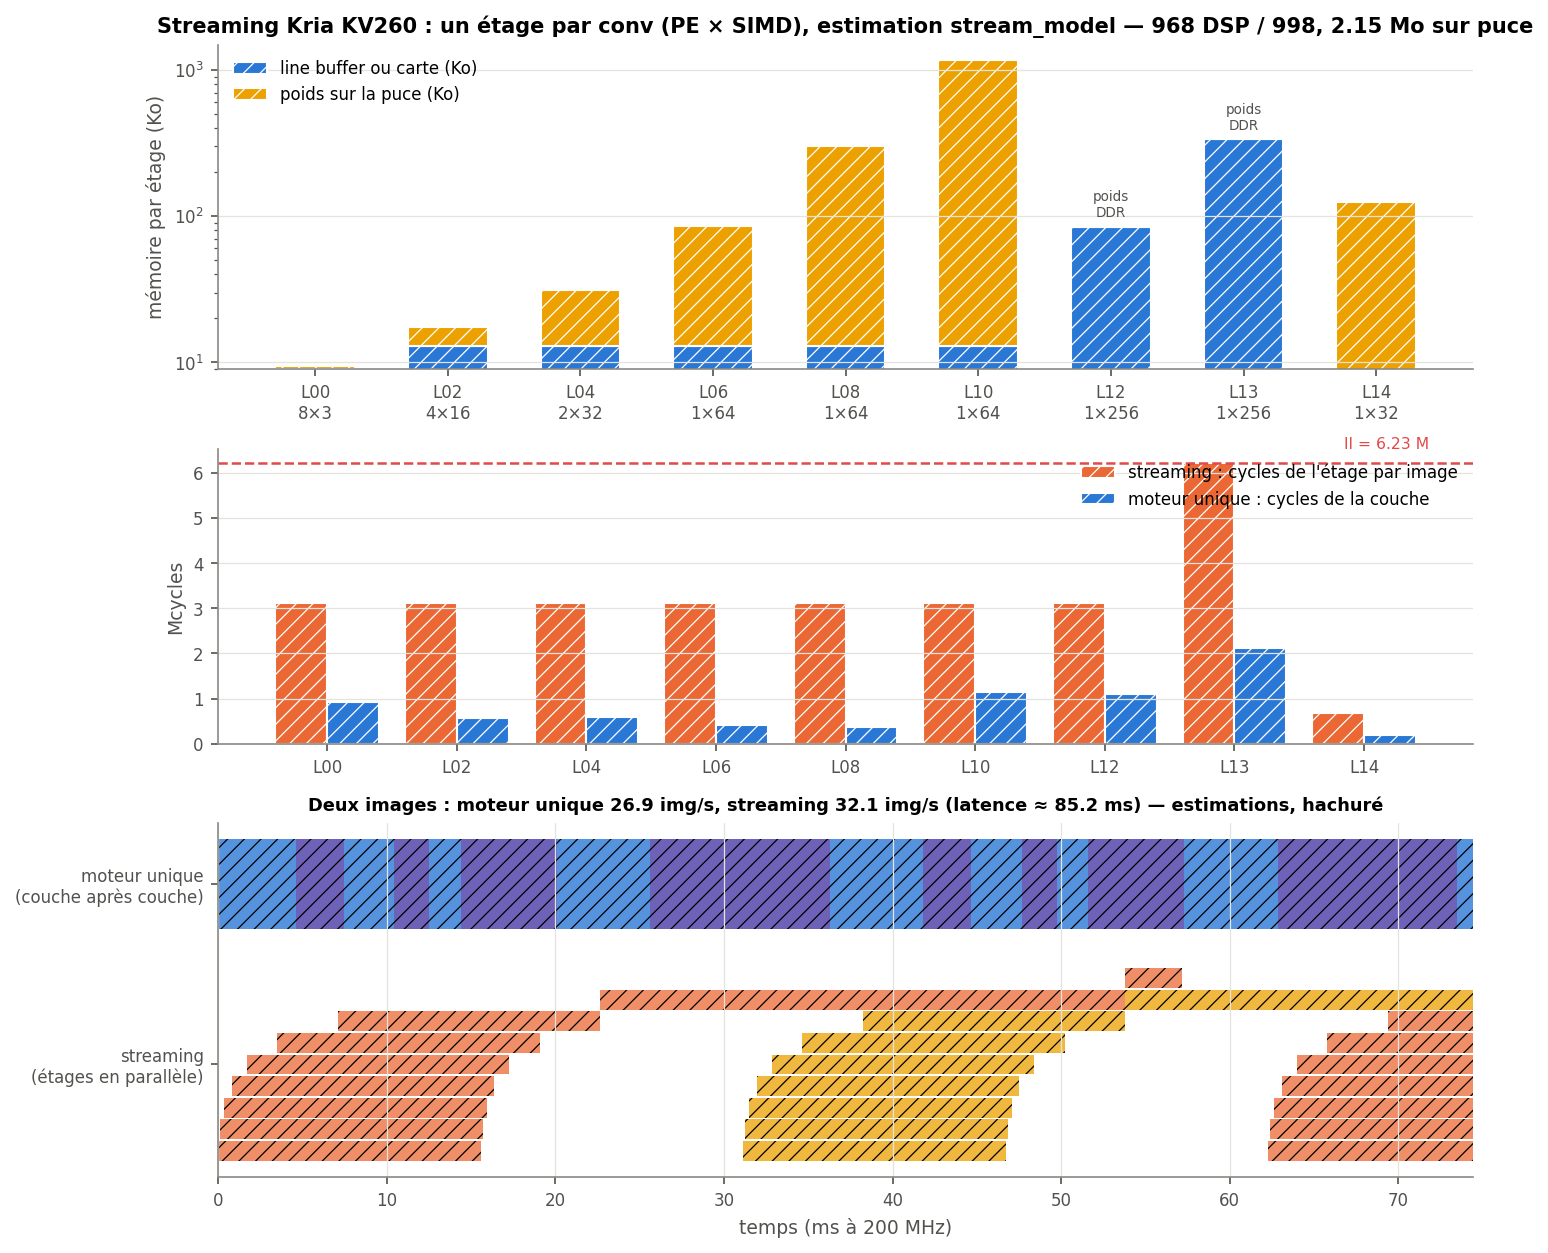
\includegraphics[width=\linewidth,height=0.42\textheight,keepaspectratio]{../../results/figures/materiel/streaming.png}
\caption{Architecture streaming face au moteur unique : mémoire et parallélisme par étage, cycles par couche, chronogramme sur deux images (estimations). (\texttt{streaming})}
\label{fig:streaming}
% python -m tools.figures streaming
\end{figure}}
\expandafter\def\csname artfig:detections\endcsname{%
\begin{figure}[htbp]
\centering
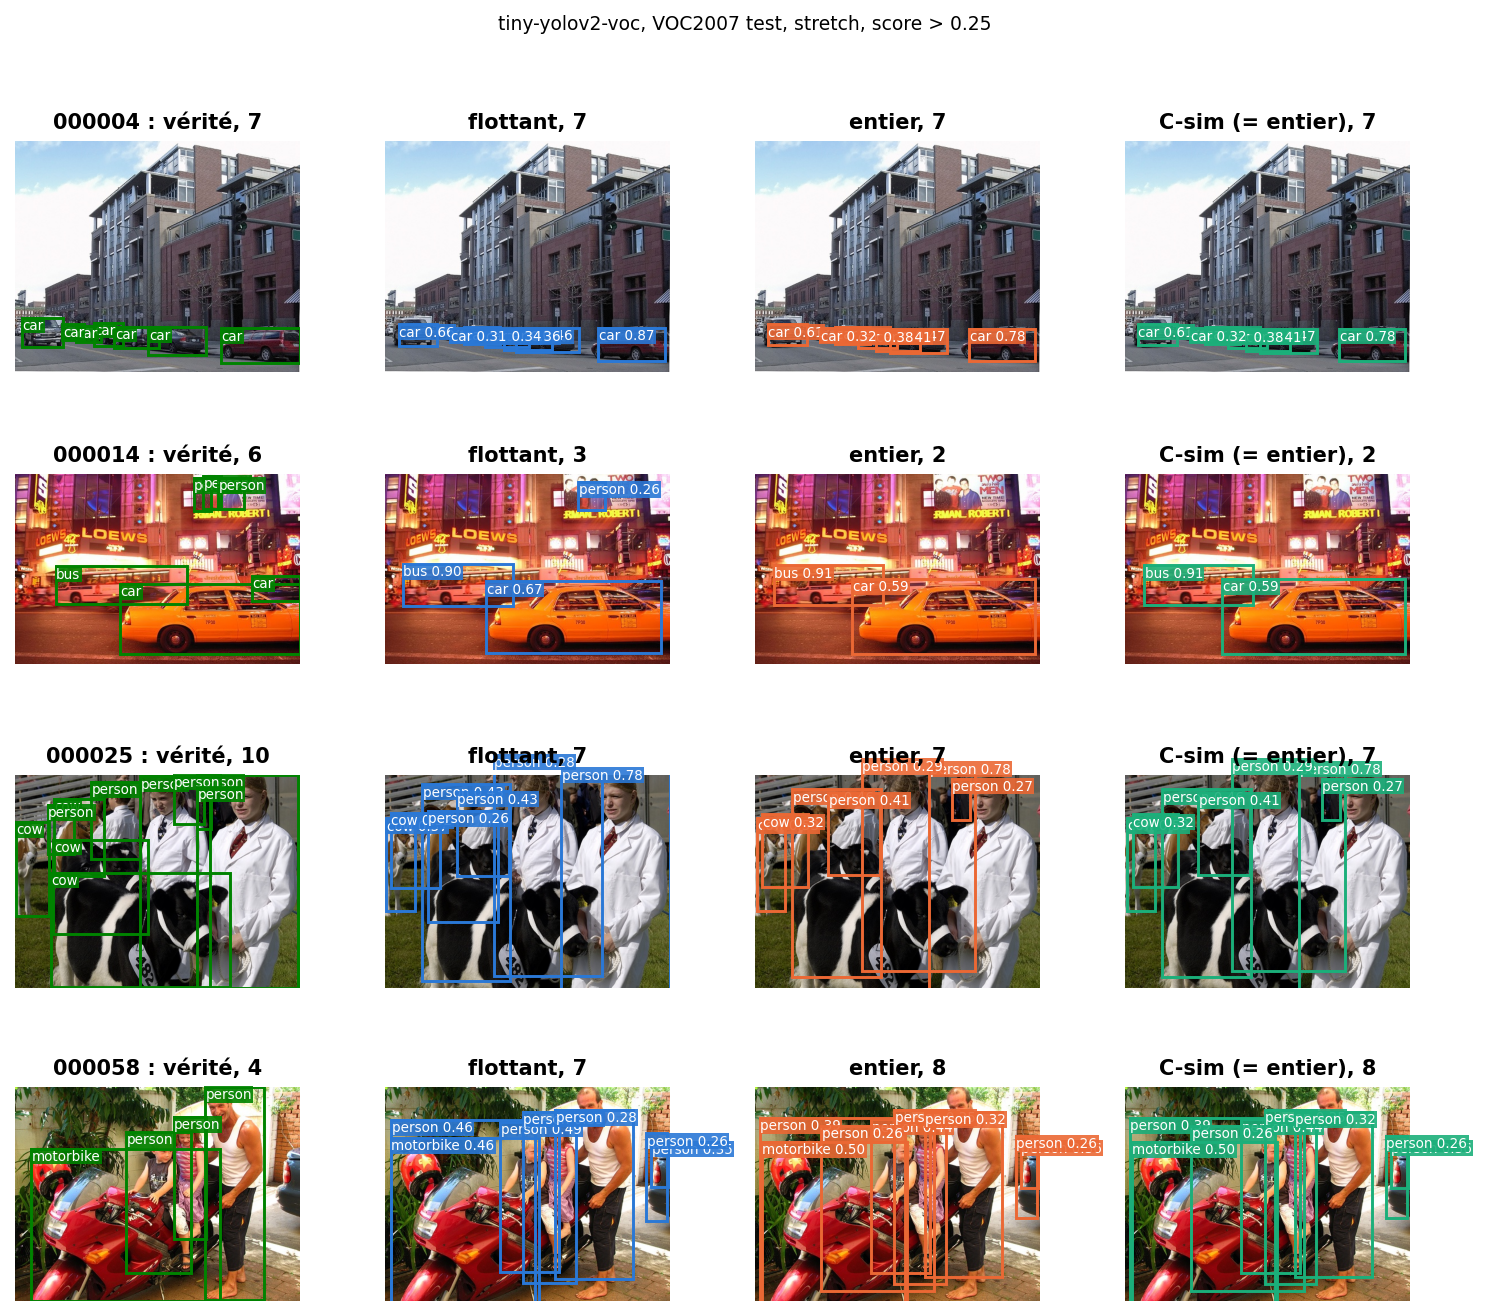
\includegraphics[width=\linewidth,height=0.42\textheight,keepaspectratio]{../../results/figures/resultats/detections.png}
\caption{Vérité terrain, flottant, entier et C-sim sur quatre images de VOC2007 test : les colonnes entier et C-sim sont identiques. (\texttt{detections})}
\label{fig:detections}
% python -m tools.figures detections
\end{figure}}
\expandafter\def\csname artfig:tests\endcsname{%
\begin{figure}[htbp]
\centering
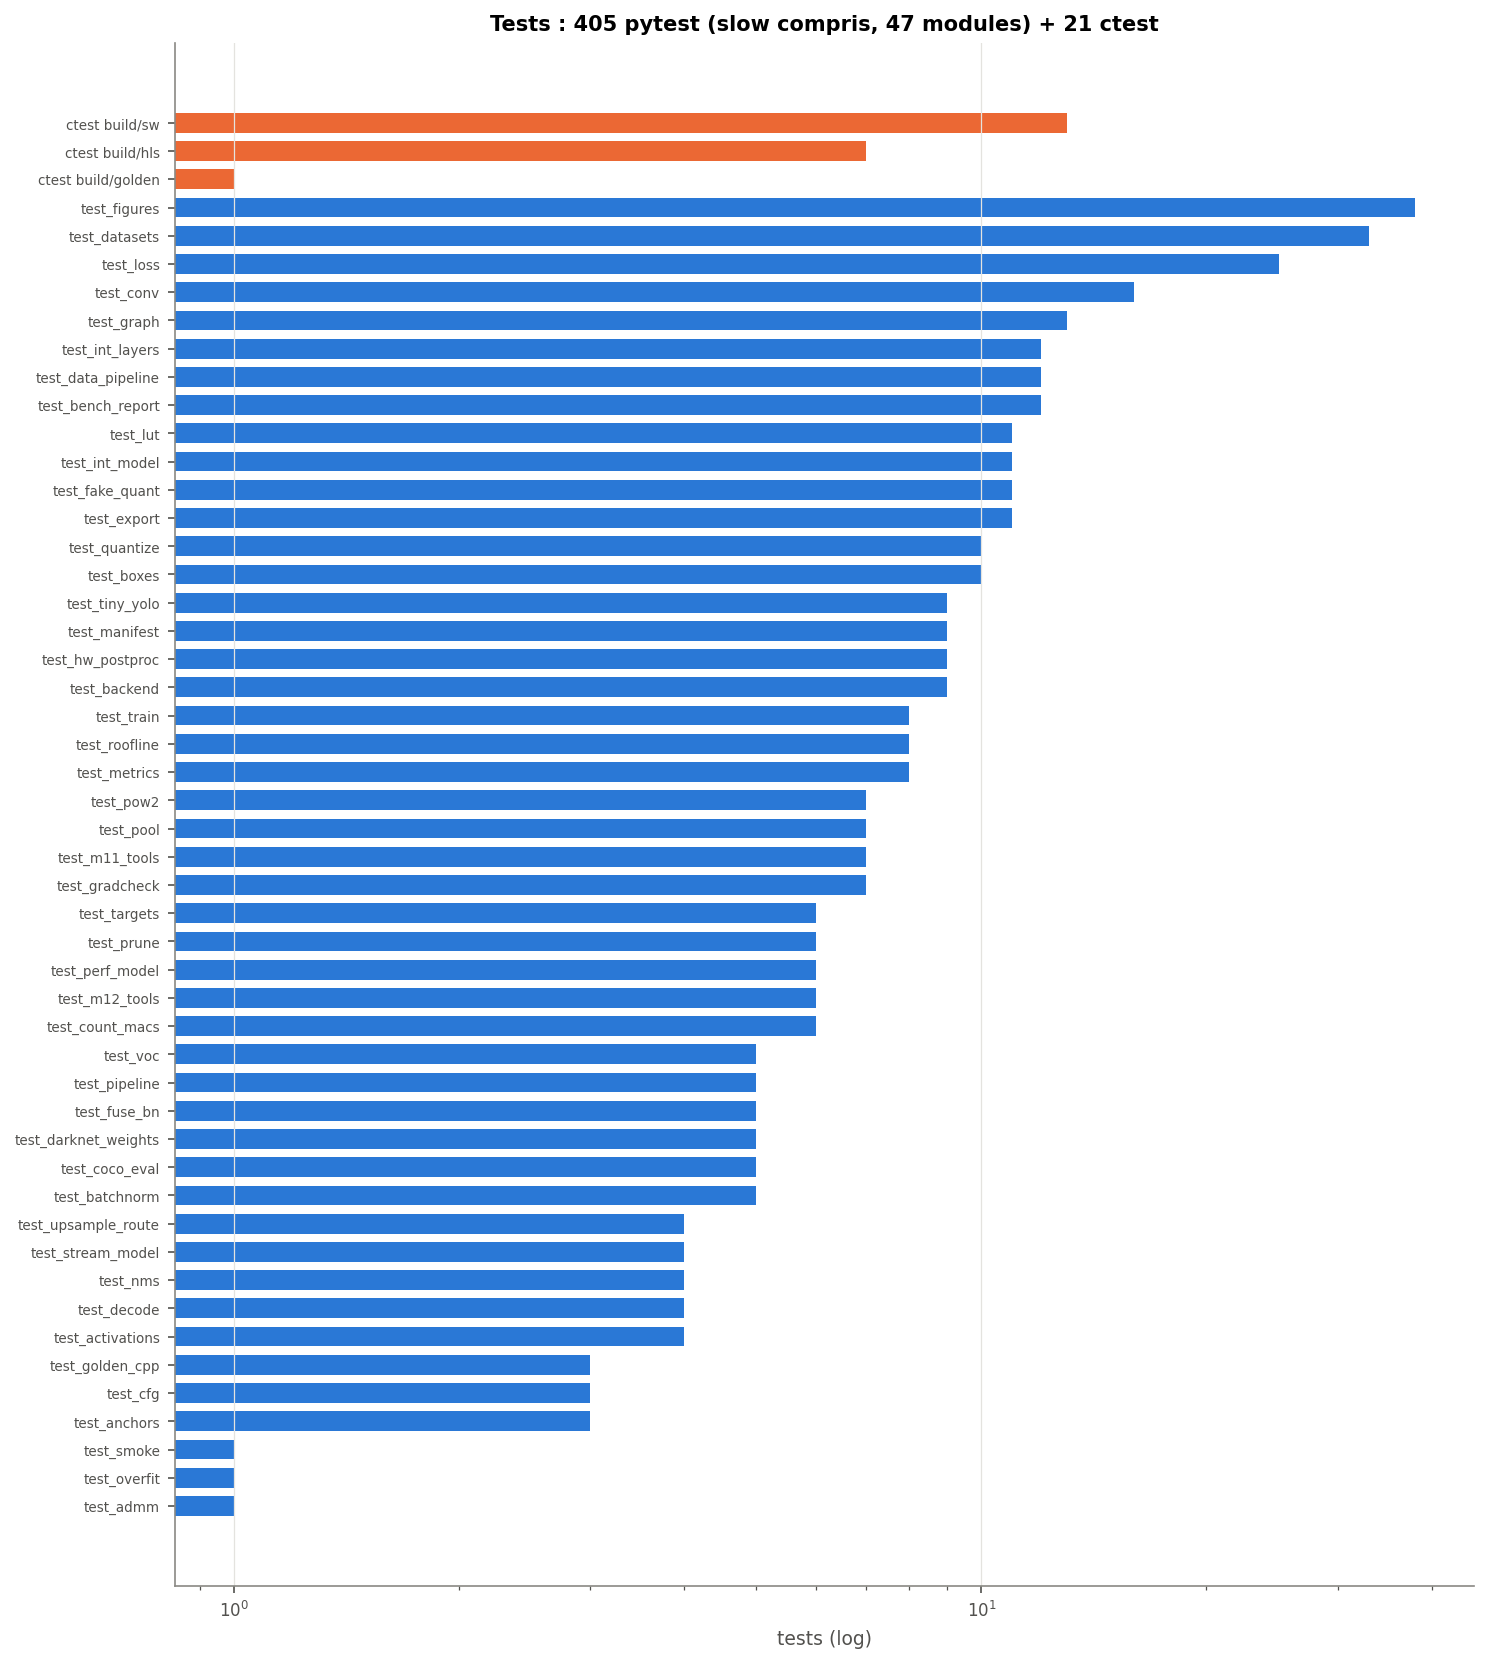
\includegraphics[width=\linewidth,height=0.42\textheight,keepaspectratio]{../../results/figures/projet/tests.png}
\caption{Nombre de tests par module Python (pytest, slow compris) et par build C++ (ctest), et leur durée quand \texttt{make test-durations} a été lancé. (\texttt{tests})}
\label{fig:tests}
% python -m tools.figures tests
\end{figure}}
\expandafter\def\csname artfig:code\endcsname{%
\begin{figure}[htbp]
\centering
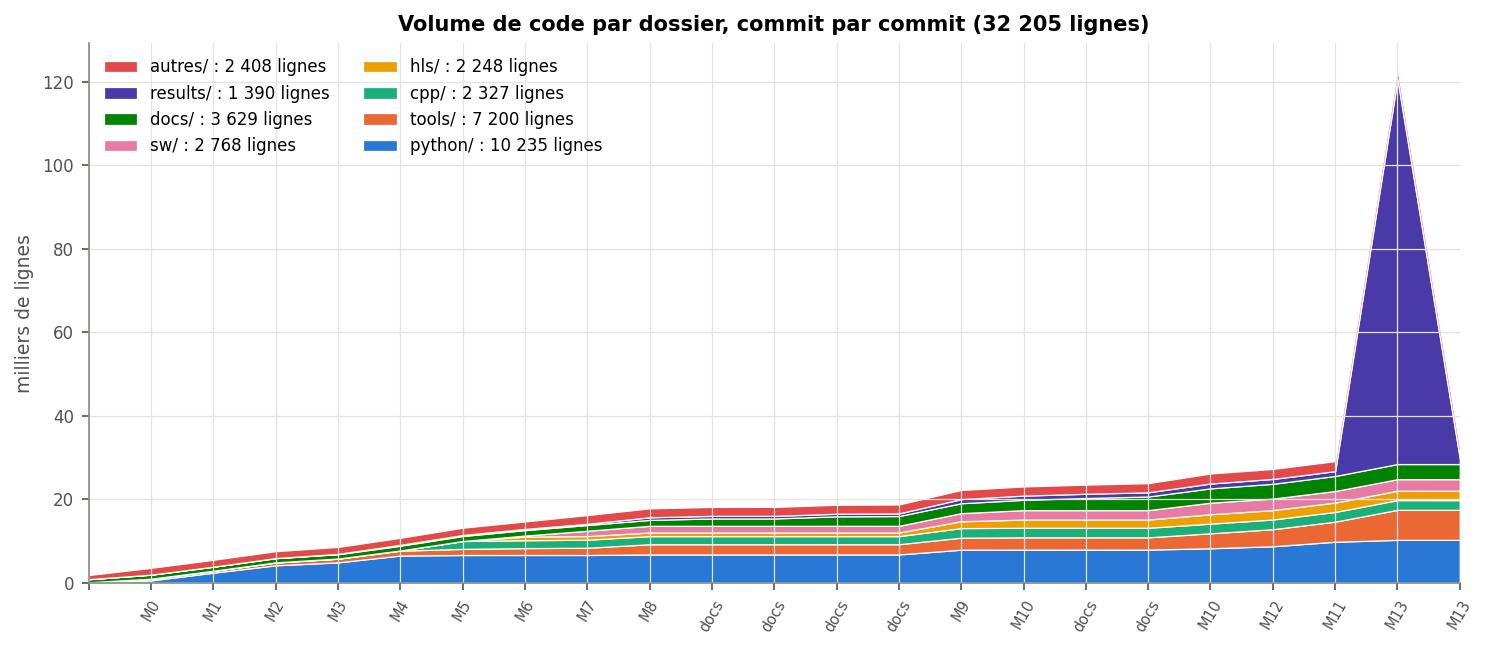
\includegraphics[width=\linewidth,height=0.42\textheight,keepaspectratio]{../../results/figures/projet/code.png}
\caption{Lignes par dossier (python, tools, cpp, hls, sw, docs, results) commit par commit. (\texttt{code})}
\label{fig:code}
% python -m tools.figures code
\end{figure}}
% ---- milestones, pending keys, revision
\newcommand\articleetat{%
\begin{tabular}{@{}lrrr@{}}
\toprule
\textbf{Milestone} & \textbf{Tasks} & \textbf{Done} & \textbf{Progress} \\
\midrule
M0 & 6 & 6 & 100\,\% \\
M1 & 9 & 8 & 89\,\% \\
M2 & 9 & 8 & 89\,\% \\
M3 & 4 & 4 & 100\,\% \\
M4 & 7 & 7 & 100\,\% \\
M5 & 6 & 6 & 100\,\% \\
M6 & 6 & 1 & 17\,\% \\
M7 & 4 & 0 & 0\,\% \\
M8 & 3 & 0 & 0\,\% \\
M9 & 1 & 0 & 0\,\% \\
M9.1 & 3 & 2 & 67\,\% \\
M9.2 & 4 & 3 & 75\,\% \\
M9.3 & 5 & 5 & 100\,\% \\
M9.4 & 3 & 3 & 100\,\% \\
M10 & 13 & 0 & 0\,\% \\
M12 & 11 & 0 & 0\,\% \\
M11 & 8 & 0 & 0\,\% \\
M13 & 54 & 54 & 100\,\% \\
M14 & 12 & 5 & 42\,\% \\
M15 & 16 & 1 & 6\,\% \\
M16 & 19 & 17 & 89\,\% \\
M17 & 21 & 17 & 81\,\% \\
M18 & 11 & 8 & 73\,\% \\
M19 & 12 & 0 & 0\,\% \\
\midrule
\textbf{Total} & \textbf{247} & \textbf{155} & \textbf{63\,\%} \\
\bottomrule
\end{tabular}}
\newcommand\articleetatresume{155 of 247 tasks done across 24 milestones, 7 milestones complete}
\newcommand\articlestatuslist{%
{\raggedright
\begin{itemize}
\item \textbf{projection} (10): \texttt{perf.cascade}, \texttt{perf.kv260}, \texttt{perf.kv260.bound.ms}, \texttt{perf.kv260.m6.ms}, \texttt{perf.kv260.roofline.ms}, \texttt{perf.kv260.v2.eff}, \texttt{perf.kv260.v2.fps}, \texttt{perf.kv260.v2.gops}, \texttt{perf.kv260.v2.ms}, \texttt{perf.kv260.v3.ms}
\item \textbf{estimate} (4): \texttt{stream.w4.fps}, \texttt{stream.w8.dsp}, \texttt{stream.w8.fps}, \texttt{stream.w8.latency}
\item \textbf{tier-R} (9): \texttt{balayage.crowdhuman.meilleur.map}, \texttt{balayage.exdark.meilleur.map}, \texttt{balayage.flir.meilleur.map}, \texttt{balayage.kitti.meilleur.map}, \texttt{balayage.visdrone.meilleur.map}, \texttt{balayage.voc.meilleur.map}, \texttt{balayages.meilleurs}, \texttt{quant.sensitive.gap}, \texttt{quant.sensitive.layer}
\item \textbf{csim} (3): \texttt{map.voc.csim}, \texttt{map.voc.identical}, \texttt{verif.hwpp.cases}
\end{itemize}\par}}
\newcommand\articlerev{rev.~\texttt{07c97e1-dirty}, 2026-10-07}
